\documentclass[11pt]{scrreprt}

\renewcommand{\textfraction}{0.001}
\renewcommand{\topfraction}{0.999}   
\renewcommand{\bottomfraction}{0.999}

\usepackage{graphicx}
\usepackage{amsmath}
\usepackage{mathtools}
\usepackage{amssymb}
\usepackage[bibencoding=utf8, backend=biber, style=numeric-comp, sorting=none, minbibnames=1, maxnames=5]{biblatex}
\addbibresource{bibliography.bib}
\usepackage{a4,color}
\usepackage{tikz}
\usepackage{pgfplots}
\pgfplotsset{compat=1.10}
\usepackage{calc}

\usepackage{booktabs,multirow}
\usepackage{newfloat}
\usepackage{caption}
\usepackage{longtable}
% \usepackage{subcaption}
\usepackage{float}
\usepackage{url}
\usepackage{listings}
\usepackage{hyperref}
\usepackage{subfig}
\usepackage[top=3.5cm, bottom=3.5cm, left=3cm, right=3cm]{geometry}

\usepackage[T1]{fontenc}
\usepackage[utf8]{inputenc}

\usepackage{mathpazo}

\definecolor{red}{rgb}{1,0,0}
\definecolor{green}{rgb}{0,1,0}
\definecolor{blue}{rgb}{0,0,1}
\definecolor{darkblue}{rgb}{0,0,0.8}

\definecolor{yellow}{rgb}{1,1,0}
\definecolor{lightblue}{rgb}{0,1,1}
\definecolor{magenta}{rgb}{1,0,1}
\definecolor{lightgrey}{rgb}{0.5,0.5,0.5}
\definecolor{grey}{rgb}{0.35,0.35,0.35}
\definecolor{darkgrey}{rgb}{0.2,0.2,0.2}
\definecolor{ockerrot}{rgb}{0.859,0.375,0.152}

% Default fixed font does not support bold face
\DeclareFixedFont{\ttb}{T1}{txtt}{bx}{n}{12} % for bold
\DeclareFixedFont{\ttm}{T1}{txtt}{m}{n}{12}  % for normal

% Custom colors
\usepackage{color}
\definecolor{deepblue}{rgb}{0,0,0.5}
\definecolor{deepred}{rgb}{0.6,0,0}
\definecolor{deepgreen}{rgb}{0,0.5,0}

\usepackage{listings}

% Python style for highlighting
\lstset{
language=Python,
basicstyle=\ttm,
otherkeywords={self, for},             % Add keywords here
keywordstyle=\ttb\color{deepblue},
emph={MyClass,__init__, np},          % Custom highlighting
emphstyle=\ttb\color{deepred},    % Custom highlighting style
stringstyle=\color{deepgreen},
frame=tb,                         % Any extra options here
showstringspaces=false            % 
}

\DeclareFloatingEnvironment[fileext=cds,placement={!ht},name=Code Snippet]{codesnippet}

\captionsetup{margin=0pt,font=small,labelfont=sc,labelformat=simple,format=plain,indention=3mm,
 labelsep=endash,textfont=sf,font=sf,singlelinecheck=on,figurename=Fig.,tablename=Tab.}

\captionsetup[codesnippet]{margin=0pt,font=small,labelfont=sc,labelformat=simple,format=plain,indention=3mm,
 labelsep=endash,textfont=sf,font=sf,singlelinecheck=on}

\fontfamily{ppl}\selectfont

\newcommand*{\bfrac}[2]{\genfrac{\big (}{\big )}{0pt}{}{#1}{#2}}

\setlength{\parskip}{1.5ex plus 0.5ex minus 0.2ex}
\setlength{\parindent}{0pt}

% \linespread{1.5}\selectfont

\begin{document}


\begin{titlepage}
  \includegraphics[width=0.4\textwidth]{pics/uzh_logo_e_pos.pdf}
  \vspace{1cm}

  \Huge\centering New Approach for a Circle Hough Transform to Detect
        Cherenkov Rings in the LHC\textit{b} RICH detector 

  \noindent\makebox[\textwidth]{\rule{\textwidth}{0.4pt}}

\vspace{1cm}

{\centering
  \Large Master thesis\\
  of\\
  Philipp Gloor
  \vspace{1.5cm}

  \Large Mathematisch-naturwissenschaftliche Fakultät\\
  der\\
  Universität Zürich
  \vspace{2cm}

  \Large 
  Prof. Dr. P. Saha\\
  Prof. Dr. U. Straumann\\
  Dr. O. Steinkamp\\
\vspace*{\fill}
\Large Zürich 2016


  }
\end{titlepage}
\chapter*{Abstract}
\addcontentsline{toc}{chapter}{Abstract}
This thesis explores possible algorithms for the detection of rings of Cherenkov photons which are produced by particles 
travelling through a RICH detector in the LHC\textit{b} experiment. These rings can be detected with the help of a Hough 
transform. After a brief introduction to LHC\textit{b} and the RICH detector, this thesis gives a short introduction to 
the linear Hough transform (which detects straight lines) to give a rough idea about what a Hough transform can do. 
This is followed a brief look at the circle Hough transform (which detects circles). This part is split in 3 sections, 
discussing 1D, 2D and 3D Hough transforms. The 1D Hough transform can be used when the center of the circle is given and only its radius 
needs to be found. The 2D Hough transform looks for the position of circle centers ($(x,y)$ coordinate) for a given radius. 
The 3D Hough transform is used when neither center nor radius of the ring are known. This is the case for the data from LHC\textit{b} 
where there are data points (photons from several Cherenkov rings and noise hits) and the algorithm has to find all the rings.

Apart from the standard Hough transform with a 3D accumulator space this thesis develops a new approach for a Hough transform. 
This approach works on the basis that each circle is defined by 3 points. Given 3 points one can calculate the circumcenter 
(the center of the circle we are intersted in) and the radius of the circumcircle.

\tableofcontents
\listoftables
\listoffigures	
\listofcodesnippets

\chapter{Introduction}
\section{LHC - Large Hadron Collider} % (fold)
\label{sec:lhc_large_hadron_collider}
\begin{figure}[htb]
  \centering
  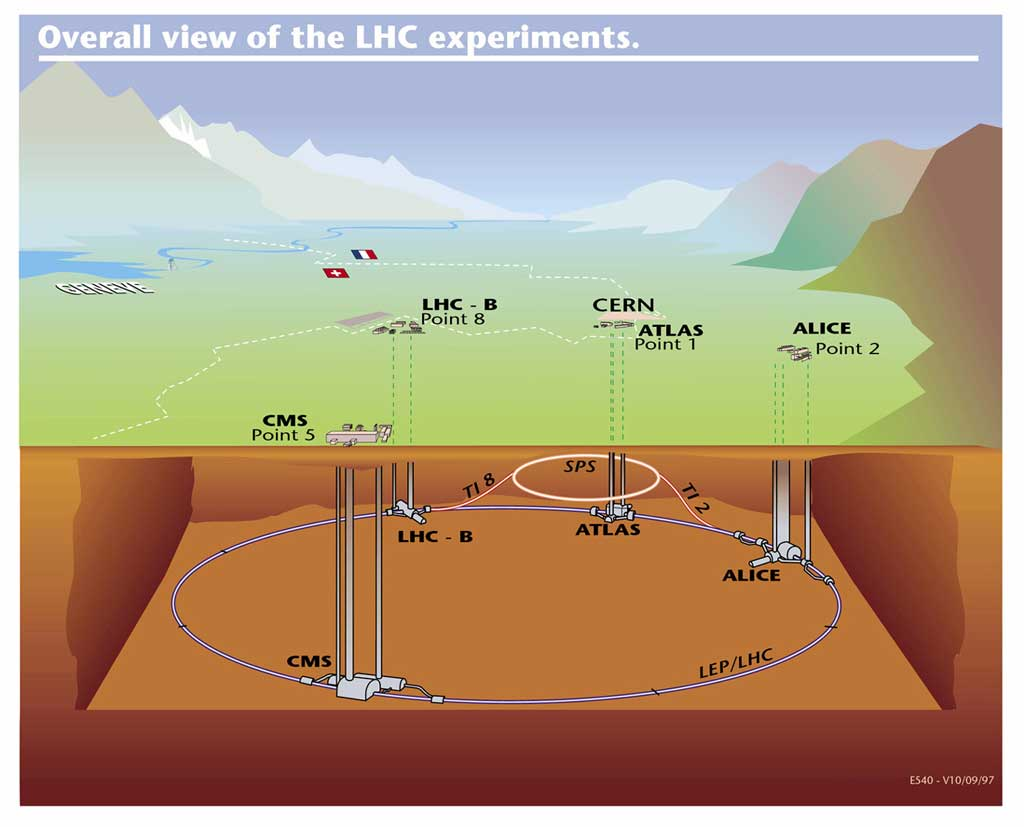
\includegraphics[width=0.6\textwidth]{pics/lhc}
  \caption{The LHC ring with its four large experiments: ATLAS, CMS, ALICE and LHC\textit{b}}
  \label{fig:lhc}
\end{figure}

The Large Hadron Collider (LHC) is the largest and highest-energy particle accelerator in the world colliding protons on protons
at beam energies of up to $6.5$\,TeV and lead ions at beam energies up to $5.5$\,GeV/nucleon. It was built by the European 
Organisation for Nuclear Research (CERN) from 1998 to 2008. It aims to test the predictions of different theories in high-energy particle 
physics, in particular for the search of the Higgs boson (which has been confirmed last year) and signs for possible new physics beyond 
the Standard Model of particle physics. The LHC lies in a tunnel $27$\,km in circumference and up to $100$\,m below the surface of the 
French-Swiss border near Geneva. The LHC was built in collaboration with over 10000 scientists and engineers from over 100 countries. 
The accelerator has been running with a center of mass energy of $\sqrt{s} = 13$ TeV since 20 May 2015.

The LHC hosts four large experiments \parencite{Aad2008,Aamodt2008,AlvesJr2008,Collaboration2008}:

\paragraph{ATLAS/CMS}
  \begin{itemize}
    \item The two multi-purpose experiments at the LHC with the main goal of probing $p-p$ collisions for direct searches of new particles.
  \end{itemize}
\paragraph{ALICE}
  \begin{itemize}
    \item ALICE (A Large Ion Collider Experiment) is a general-purpose, heavy ion detector at the CERN LHC
    which focuses on QCD, the strong interaction sector of the Standard Model, e.g. searching for evidence for quark-gluon
    plasma.
  \end{itemize}
\paragraph{LHC\textit{b}}
  \begin{itemize}
    \item LHC\textit{b} is testing the Standard Model by confronting its predictions with precise measurements in CP
    violation and rare decays of particles containing $b$ and $c$ quarks.
  \end{itemize}



% section lhc_large_hadron_collider (end)

\section{The LHC\textit{b} experiment}

\begin{figure}[tb]
  \centering
  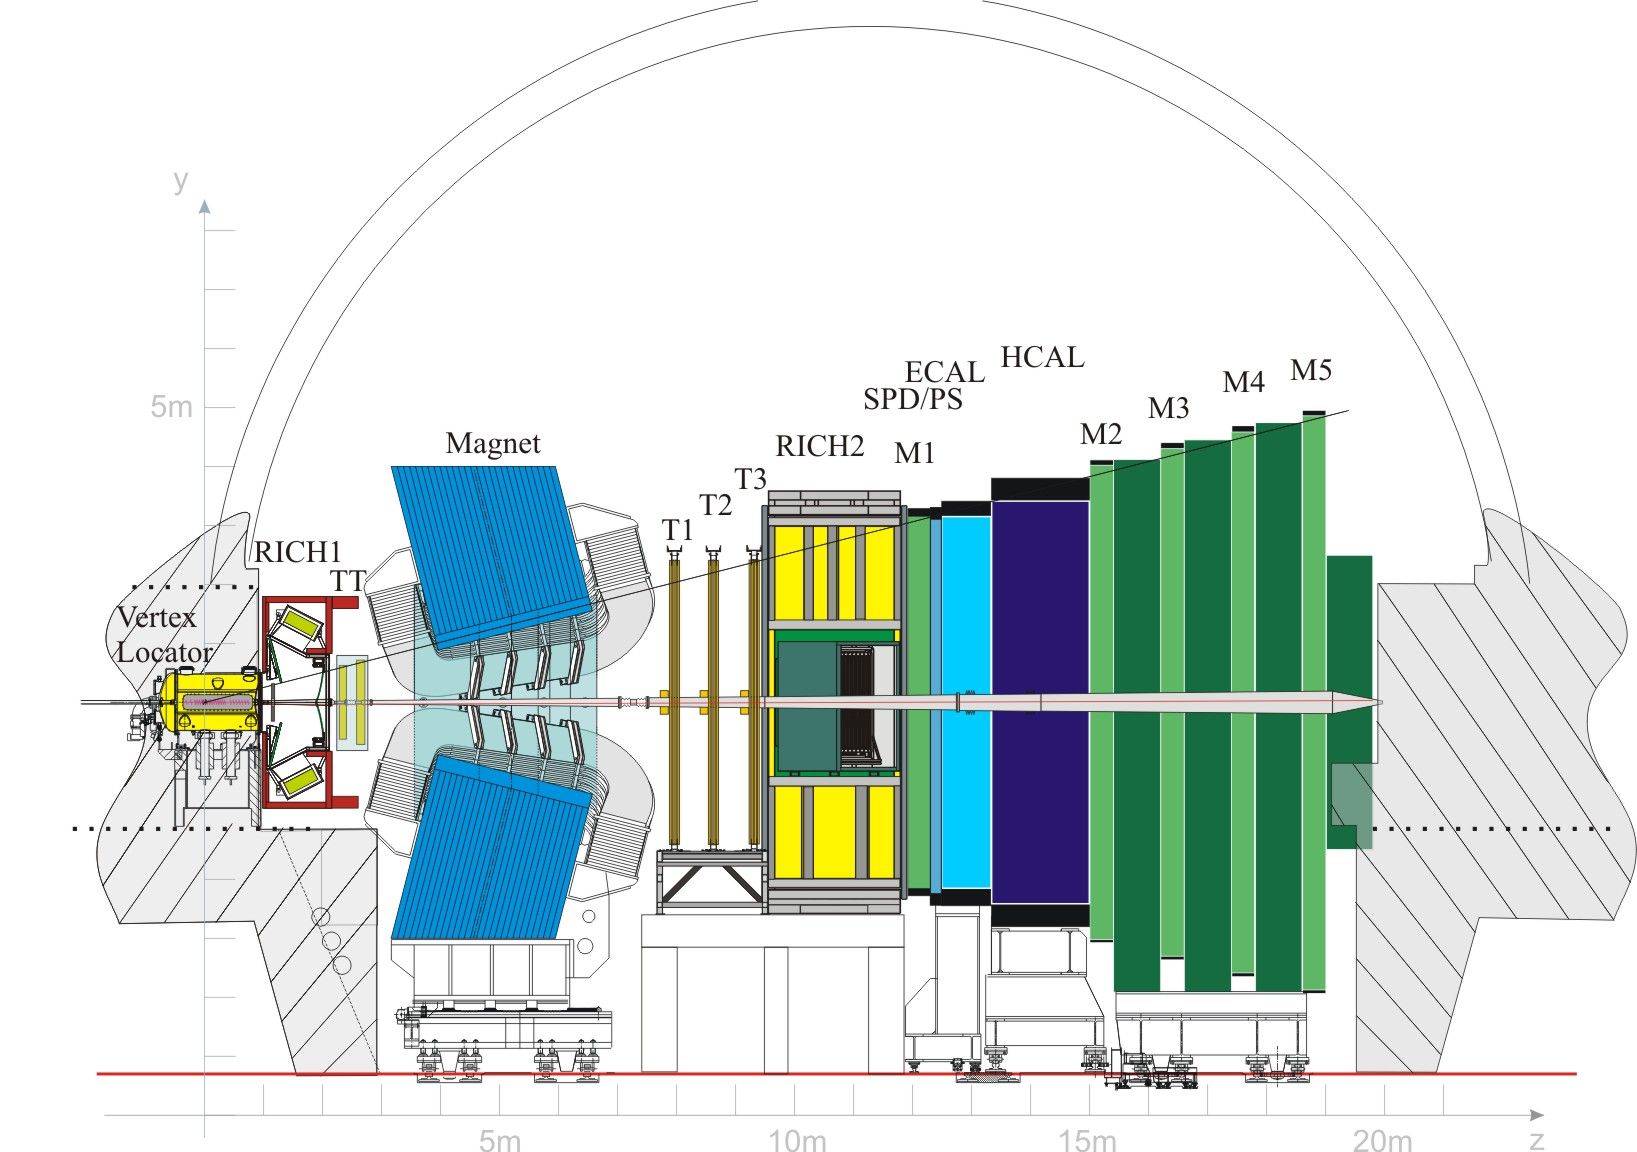
\includegraphics[width=\textwidth]{pics/lhcb_detector}
  \caption[LHC\textit{b} detector]{LHC\textit{b} Detector: The beams collide inside the Vertex Locator. The RICH1 is positioned before the tracking station (TT) and
  the magnet. RICH2 is set up after the magnet and the tracking stations (T1-T3) and before the calorimeter (SPD/PS, ECAL, HCAL) and muon stations (M1-M5)}
  \label{fig:lhcb}
\end{figure}

The main goal of the LHC\textit{b} experiment is the study of decays of particles containing $b$ and $\bar{b}$ quarks (such as \textit{B}-Mesons). During the $p-p$ collisions at the LHC these particles 
are produced mostly at small polar angles with respect to the beam axis. This is reflected in the design of the LHC\textit{b} detector 
which is a foward arm spectrometer 20 meters long with subdetectors arranged along the beam pipe as shown in figure \ref{fig:lhcb}.

A brief overview of the detector parts \parencite{lhcbweb}.

\paragraph{VELO} The VErtex LOcator surrounds the region where the beams collide and $b$/$\bar{b}$ pairs are produced. The VELO measures the 
distance between the $p-p$ collision point and the point where the \textit{B} particles decay. \textit{B} particles are short-lived (decaying after typically
$1$\,cm) thus their properties are not measured directly but inferred from the separation of these two points and the properties of 
their decay products.

\paragraph{RICH} The RICH detectors are built for particle identification in particular to distinguish charged kaons from pions. 
One detector on each side of the magnet is used to cover different momentum ranges. RICH detectors work by measuring emissions of 
Cherenkov radiation which is produced if a particle travels faster than the speed of light through a certain medium (often compared 
to breaking the sound barrier). The emission angle depends on the speed of the particle, so knowing the speed and the momentum (from the
curvature of the track induced by the magnet) the mass of the particle can be inferred.

\paragraph{Magnet} Particles normally move in a straight line but a magnetic field causes the path of charged particles to 
curve according to the Lorentz force 
\[
  \mathbf{F} = q\left( \mathbf{E} + \left( v\times\mathbf{B}\right)\right)
\]
thus allowing to determine the charge sign of the particle. Also the track curvature can be used to measure the momentum of the particle.

\paragraph{Tracking System} The tracking system is based on 4 planar tracking stations. It is used to determine the momentum of charged
particles by measuring the bending of the trajectory in the magnetic field. Two types of tracking detectors are used in LHC\textit{b}. In the silicon detector a passing particle generates electron-hole pairs which induce a charge on the readout strips. In the straw tube detector a particle ionises the gas molecules in gas-filled tubes which induce charges on a readout wire.

\paragraph{Calorimeters} They are designed to stop particles and measure their energy. The design of the stations is sandwich like with alternating metal and scintillator plates. Interactions in the metal plate cause a secondary shower of charged particles which induce scintillation light in the scintillator plates. The energy lost is proportional to the amount of light emmitted. Calorimetry is also the main way of identifying neutral particles (e.g. photons, neutrons).

\paragraph{Muon system}
Muons are easy to identify and play an important role in many analyses. There are five planar stations at the end of the detector each consisting of an iron absorber and a detection plane. The total area covered by these 
stations is about $435$\,m$^2$~\cite{Alves:2012ey}. The goal of the absorber is to stop all particles except muons who still can pass. The muons get detected 
in the gaseous detectors where their trajectory is measured.
% The fact that at the LHC b-hadrons are predominantly produced in the forward region was used in the construction of the detector. The \emph{LHC\textit{b}} experiment is a single arm forward spectrometer with a 4\,Tm dipole magnet and a polar angular coverage from 10 to 300 mrad in the horizontal plane (the bending plane of the dipole magnet) and 250 mrad in the vertical plane.


\subsection{Particle identification} % (fold)
\label{sub:particle_identification}

An important requirement at LHC\textit{b} is particle identification. This is handled by the calorimeters, Muon and RICH sub-detectors. The 
Calorimeters beside measuring energies and positions of electrons, photons and hadrons also provide identification of said particles e.g.
by measuring the shape of the induced showers. The Muon system identifies muons to a very high level of purity.
       
Hadron identification i.e. separation of kaons, pions and protons is  important for many analyses. The LHC\textit{b} RICH system 
provides this, covering a momentum range of approximately $1$--$100$\,GeV. It is composed of two detectors. One is positioned upstream of the 
dipole magnet and the other one is positioned downstream of the dipole magnet. Their setup is briefly described in Section~\ref{sec:rich_detector}.


% subsection particle_identification (end)

\chapter{Theory}

\section{Cherenkov radiation} % (fold)
\label{sec:cherenkov_radiation}

The speed of light in vacuum, \( \mathbf{c} = 299'792\,\text{km/s} \), is a universal physical constant. According to Einstein's special theory of relativity, 
\( c \) is the maximum speed at which all matter (or information) in the universe can travel. The speed at which light propagates in a 
medium is given by $\frac{c}{n}$, where $n$ is the refractive index of the medium and can be significantly less can \( c \).

Cherenkov radiation results when a charged particle travels through a dielectric medium with a speed greater than the speed of light 
through said medium. The velocity that must be exceeded is the phase velocity (\( v_{\text{Phase}} \text{ or short } v_{\text{P}} \)) 
and not the group velocity (\( v_{\text{Group}} = \frac{\partial \omega}{\partial k} \)),

\[ v_{\text{P}} = \frac{c}{n} = \frac{\lambda}{T}  =  \frac{\omega}{k}\]

where $\lambda$ is the wavelength of the light, $T$ the oscillation period, $\omega$ the angular frequency and $k$ the wavenumber.

As a charged particle travels through the medium, it disrupts the local electromagnetic field. If the particle travels slower than
the speed of light then the disturbance elastically relaxes to the equilibrium as the particle passes. However, if the particle 
travels at the speed $\beta\cdot c$ faster than the speed of light i.e. $\beta > 1/n$, the limited response speed of the medium means that a disturbance is left in the wake of the 
particle, and the energy in this disturbance radiates as a coherent shockwave.

\begin{figure}[htbp]
  \centering
    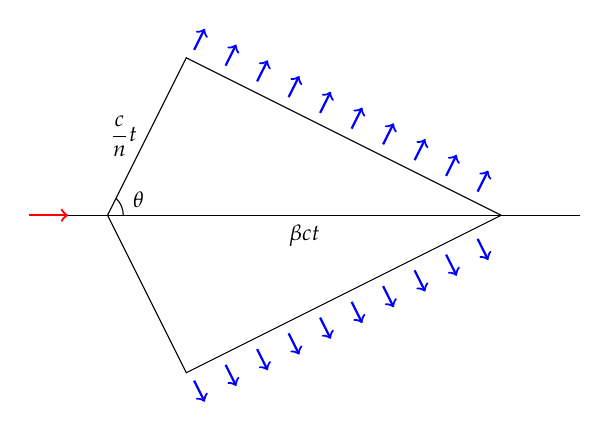
\begin{tikzpicture}
      \draw (-1,0) -- (6,0);
      \draw (0,0) -- (1,2) -- (5,0);
      \draw (0,0) -- (1,-2) -- (5,0);
      \draw[->, red, thick] (-1,0) -- (-0.5,0);
      \draw (0.2,0)arc[radius=.3,start angle=0,end angle=45];
      \node [left] at (0.5,1) {\footnotesize$\dfrac{c}{n}t$};
      \node [below] at (2.5 ,0) {\footnotesize$\beta c t$};
      \node [right] at (0.2,0.2) {\footnotesize$\theta$};
      \foreach \x in {0,1,...,9} {
        \draw[->,blue, thick] (1.1 + \x*0.4, 2.1 - \x*0.2)  --+ (63.435:0.3);
        \draw[->,blue, thick] (1.1 + \x*0.4, -2.1 + \x*0.2) --+ (-63.435:0.3);
      }
    \end{tikzpicture}
  \caption{The geometry of the Cherenkov radiation}
  \label{fig:cherenkov_radiation}
\end{figure}

As illustrated in Figure~\ref{fig:cherenkov_radiation}, the shockwave is emited under an angle
\begin{equation}
    \cos\theta = \frac{x_{\text{p}}}{x_{\text{em}}} = \frac{\frac{c}{n}t}{\beta c t} = \frac{1}{n\beta}
\end{equation}
with respect to the direction of flight of the particle. Figure~\ref{fig:radiators} shows the Cherenkov angle vs momentum for different particles and different radiators in LHC\textit{b}.

\begin{figure}[tb]
  \centering
  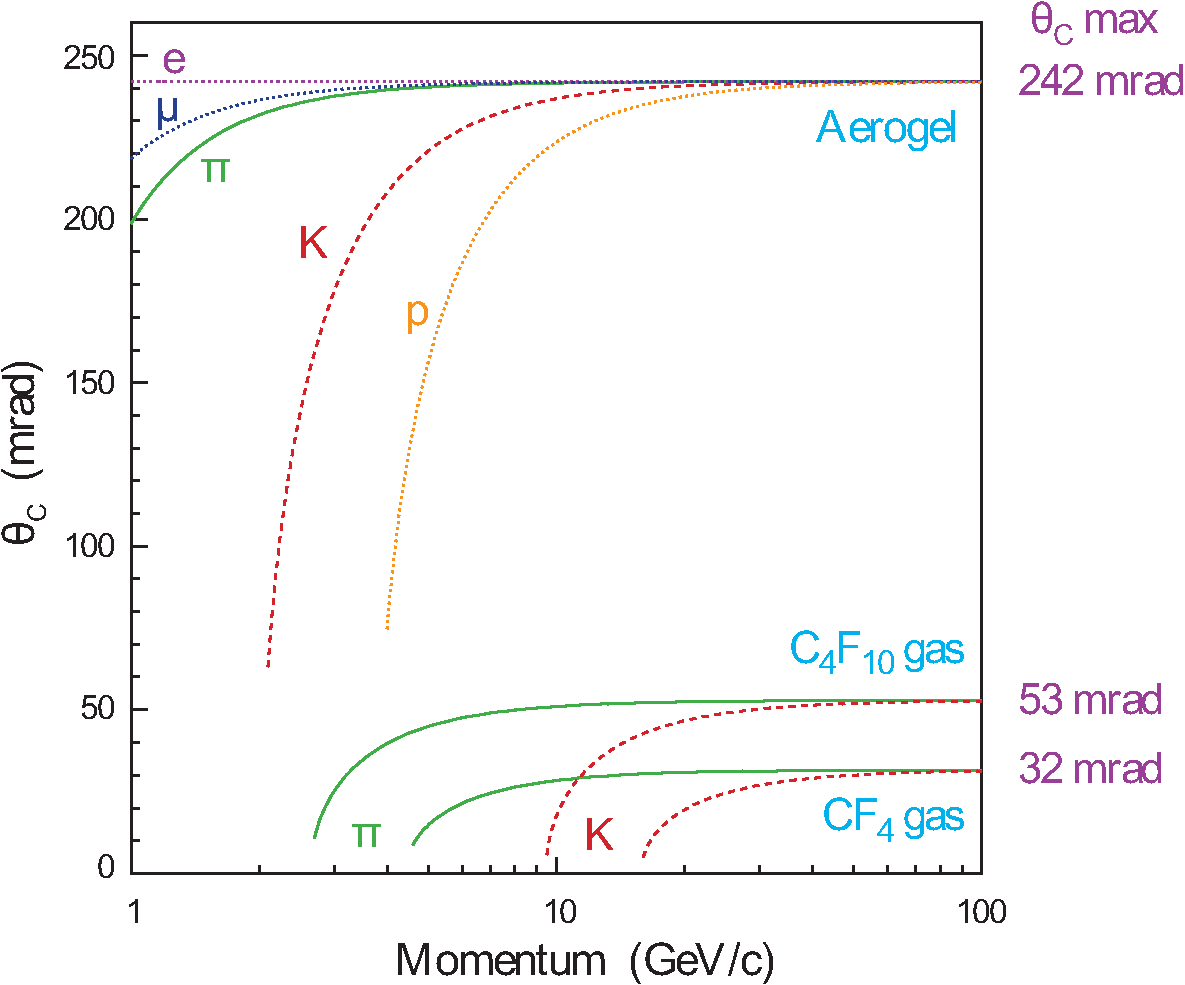
\includegraphics[width=0.8\textwidth]{pics/radiators}
  \caption{Cherenkov angle vs momentum for the different particles in different radiators}
  \label{fig:radiators}
\end{figure}

\section{RICH detector} % (fold)
\label{sec:rich_detector}

Particle identification is a fundamental requirement for many analyses at the LHC\textit{b} experiment. LHC\textit{b} is 
unique at the LHC in the sense that it uses RICH detectors for hadronic particle identification, unlike other LHC experiments such as ATLAS or CMS. The advantage of using RICH detector is that it yields superior particle identification performance. Using three different radiators, the RICH detectors cover a wide range of momentum (1-100 $\text{GeV}/c$).

Both RICH-1 and RICH-2 are located in low magnetic field regions to keep the trajectories of charged particles straight while they pass through the radiators. They both also have tilted spherical focusing primary mirrors and secondary flat mirrors to limit the length of the detector along the beam pipe and minimize the amount of detector material. The spherical focusing mirrors use the property that photons generated at a fixed angle with respect to the particle trajectory are focused onto a ring in the photon detector plane (via the secondary flat mirror) where hybrid photon detectors (HPD) are used to measure the spatial position of emitted Cherenkov photons. These photon detectors have a spatial resolution of 2.5\,mm $\times$ 2.5\,mm. The total area of the two detector planes in the RICH-1 detector is $1302$\,mm $\times 555$\,mm each and $710$\,mm $\times 1477$\,mm for RICH-2.  The HPD is a vacuum photon detector in which a photoelectron, released from the conversion in a photocathode of an incident photon, is accelerated by and applied voltage onto a silicon detector \cite{AlvesJr2008}. 

The RICH-1 in front of the magnet covers the lower momentum range from 1-60 $\text{GeV}/c$. It uses two radiators 5\,cm thick aerogel tiles with $n=1.03$ is suited for the lowest momentum tracks and directly behind about 1\,m of $\text{C}_4\text{F}_{10}$ ($n=1.0014$) which covers the intermediate region of momentum. For the highest momentum tracks, 
gaseous $\text{C}\text{F}_4$ ($n=1.0005$) is used in the RICH-2 \cite{LHCb2000}.

There is a strong correlation between the polar angle and the momentum of the charged particles produced in LHC\textit{b}. Particles with a larger polar angle tend to have lower momentum. This is why RICH-1 with the aerogel is located before the dipole magnet so tracks with low momentum will be covered before they are swept out of the acceptance by the magnet. See Figure~\ref{fig:rich1} for a schematic of the RICH-1 detector.

\begin{figure}[tb]
  \centering
  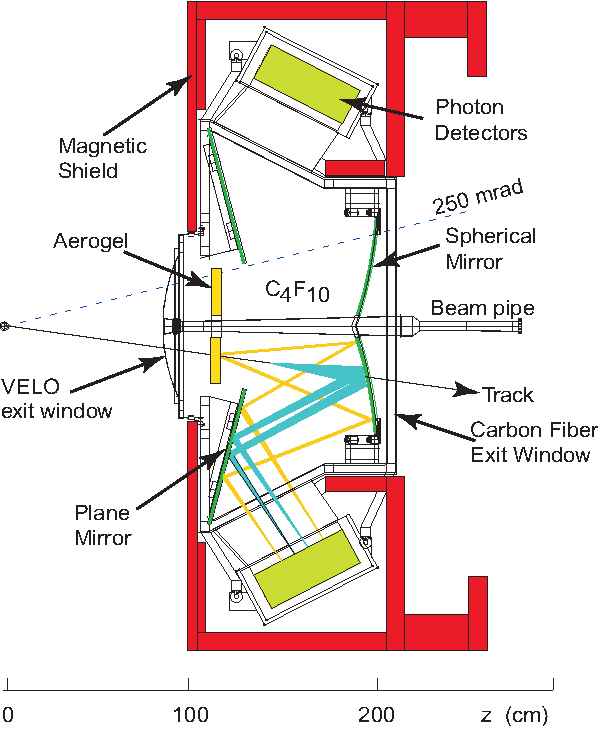
\includegraphics[width=0.5\textwidth]{pics/rich1-2d}
  \caption{RICH-1 detector \cite{LHCb:2000}}
  \label{fig:rich1}
\end{figure}


% section rich_detector (end)


% section cherenkov_radiation (end)

\section{Hough transform} % (fold)
\label{sec:hough_transform}

The Hough transform \cite{Duda:1972} is a feature extraction technique used in image analysis, computer vision and digital image processing.

Its purpose is to find imperfect instances of objects within a certain class of shapes by a voting procedure. This voting procedure is 
carried out in a parameter space from which object candidates are obtained as local maxima in a so called accumlator space that is 
explicitly constructed by the algorithm for computing the Hough transform.

Initially the Hough transform was concerned with finding straight lines \cite{c1962method} but it has been extended to identifying positions 
of more complicated shapes, such as circles and ellipses.

\subsection{Linear Hough transform} % (fold)
\label{sub:linear_hough_transform}

A linear function is often parametrized as:

\[
  f(x) = m\cdot x + b
\]
where $m$ is the slope of the line and $b$ the intercept. For the Hough transform, however, this representation is not ideal. For a 
vertical line, $m$ would go to infinity which gives an unbound parameter space for $m$. For this reason, Duda and Hart suggested the 
$r\text{-}\theta$ parametrization \parencite{Duda:1972}.

\begin{equation}
  r = x\cos\theta + y\sin\theta\label{eq:param_eq}
\end{equation}

where $r$ is the distance from the origin to the closest point on the line and $\theta$ is the angle between the $x$-axis and the line 
connecting the origin with that closest point.

\begin{figure}[ht]
  \centering
  \begin{tikzpicture}[scale=3]
    \draw[<->] (0,1.5) -- (0,0) -- (1.5,0);
    \node [left] at (0,1.5) {$y$};
    \node [below] at (1.5,0) {$x$};
    \draw[magenta,semithick] (0,1) -- (1,0);
    \draw[-> ,semithick] (0,0) -- (0.5, 0.5);
    \draw[semithick] (0.2,0) arc (0:45:0.2cm);
    \node[below] at (0.1,0.121) {\footnotesize$\theta$};
    \node[above] at (0.2,0.2) {$r$};
  \end{tikzpicture}
  \caption{$r\text{-}\theta$ parametrisation}
  \label{fig:rhotheta}
\end{figure}
% subsection linear_hough_transform (end)

This means given a single point in the ($x,y$) plane, the set of all lines going through this point form a sinusoidal curve in 
$r\text{-}\theta$ space. Another point that lies on the same straight line in the ($x,y$) plane will produce a sinusoidal curve that 
intersects with the other at ($r\text{-}\theta$) and so do all the points lying on the same straight line. 


\begin{figure}[tb]
  \centering
  \includegraphics[width=0.8\textwidth]{sim_pics/line_ht_paramspace}
  \caption[Example of a linear HT space]{This is the accumulator space of 3 points on the same line. Each curve represents line drawn through one particular point - REPHRASE THIS}
  \label{fig:line_ht}
\end{figure}

\begin{figure}[tb]
  \centering
  \includegraphics[width=0.8\textwidth]{sim_pics/line_ht_paramspace_nomatch}
  \caption[Example of a linear HT where points don't lie on a line]{Example of a linear Hough transform where points don't lie on a line. Since any 
  two points can form a line there are still intersections but never more than 2.}
  \label{fig:line_ht_nomatch}
\end{figure}

\subsection{Circle Hough transform} % (fold)
\label{sub:circle_hough_transform}

For this thesis we are interested in circle detection so we need to adapt the linear Hough transform in order to find circles. 
In a two dimensional space ($x,y$), a circle can be described by:

\begin{equation}
		(x-c_x)^2 + (y-c_y)^2 = r^2
\end{equation}

Where $(c_x,c_y)$ are the coordinates of the center of the circle and $r$ its radius. The possible parameters for the parameters space are now $c_x, c_y$ and $r$. This means if the center of the circle is known the parameter space is one-dimensional, if the radius of the circle is known the parameter space is two-dimensional and of course if nothing is known the parameter space is three-dimensional.



% subsection circle_hough_transform (end)
% section hough_transform (end)

\section{Datasets} % (fold)
\label{sec:dataset}
Two Monte-Carlo generated sets of simulated data were used for this thesis. The algorithms were trained on a data set of 250 simulated events and the performance of the algorithms was tested on a data set consisting of 10'000 simulated events with a total of 49'979 rings across all events. The properties of these events (radiuses, number of points per ring, number of rings per event) are taken from both simulation of LHC\textit{b} events and
real data taken from the experiment. The number of points per ring is determined by the photoelecton yield N$_\text{pe}$ which is shown in Table~\ref{tab:results}. Figure~\ref{fig:ppc1} shows the number of points per circle and Figure~\ref{fig:circlePerEventDist} the number of circles per event for the test data set.

\begin{table}[tb]
\centering
\begin{tabular}{c c c}
\toprule
\multirow{2}{*}{Radiator} & \multicolumn{2}{c}{Average N$_{\text{pe}}$ from data} \\
\cmidrule{2-3} &  tagged D$^0 \rightarrow$ K$^- \pi^+$ &pp$ \rightarrow$ pp $\mu^+ \mu^-$ \\
\midrule
Aerogel & $5.0 \pm 3.0$  & $4.3 \pm 0.9$\\
C$_4$F$_{10}$  & $20.4 \pm 0.1$ & $24.5 \pm 0.3$ \\
CF$_4$ & $ 15.8 \pm 0.1$  & $ 17.6 \pm 0.2$ \\ 
\bottomrule
\end{tabular}
\caption[Comparison of photoelectron yields (N$_{\rm pe}$)]{Comparison of photoelectron yields (N$_{\rm pe}$) determined from
D$^* \rightarrow$D$^0\pi^+$ decays and pp $\rightarrow$ pp $\mu^+ \mu^-$ events in data, using the selections and 
methods described in the text \cite{RICHPerf2012}}
\label{tab:results}
\end{table}

\begin{figure}[tb]
  \centering
  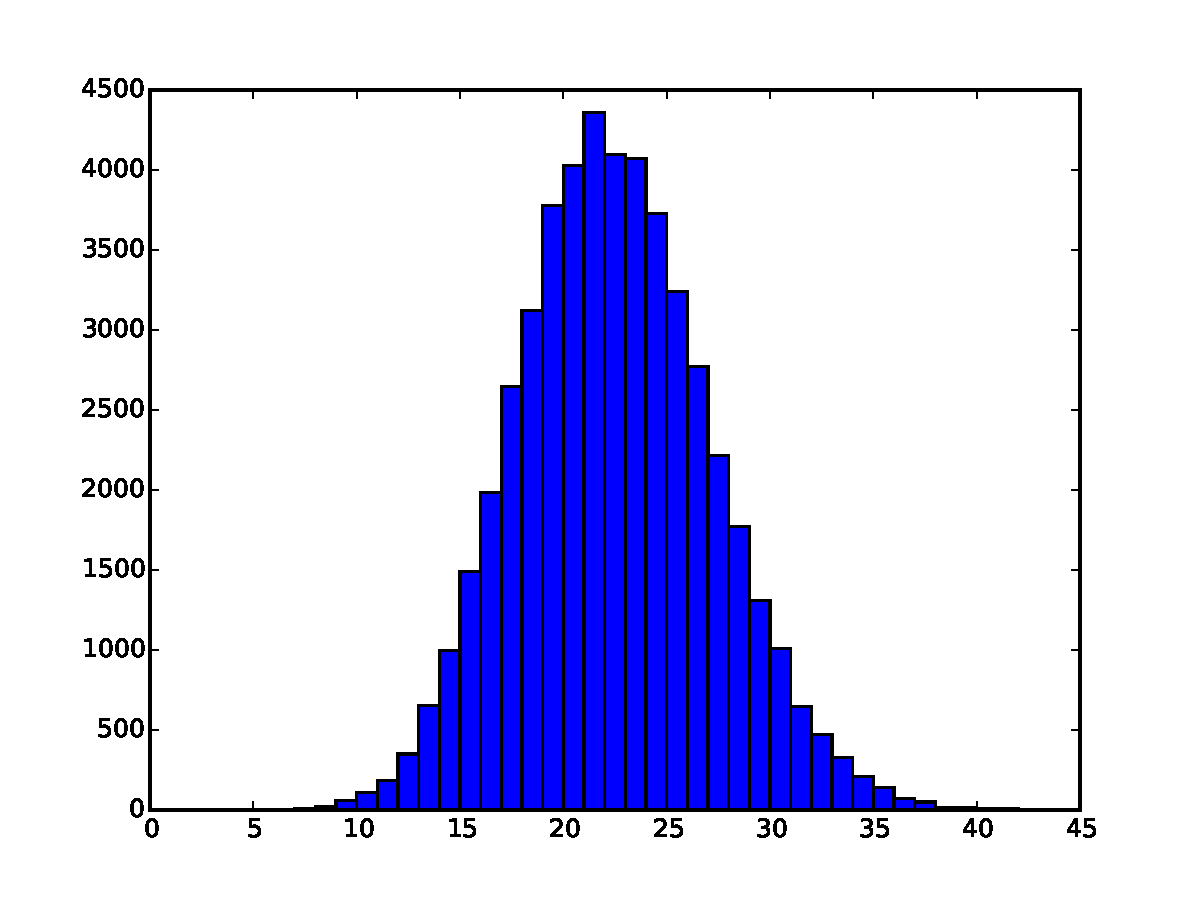
\includegraphics[width=0.6\textwidth]{sim_pics/ppc}
  \caption{Number of points per circle (N$_\text{pe}$) for the 10'000 simulated events in the test data sample}
  \label{fig:ppc1}
\end{figure}

\begin{figure}[tb]
  \centering
  \includegraphics[width=0.6\textwidth]{sim_pics/circlePerEventDistribution}
  \caption{Number of circles per event in the test data sample}
  \label{fig:circlePerEventDist}
\end{figure}

The average radius of Cherenkov rings can be found in \cite{Forty1999}. Rings from the C$_4$F$_{10}$ radiator in RICH-1 have radiuses generally smaller than $0.15$\,m. Rings from the aerogel have slightly bigger radiuses of around $0.20$\,m). All generated rings in the test data set have a radius that is smaller than $0.15$\,m. The distribution of the radiuses in the test data set is shown in Figure~\ref{fig:radius_dist}.

\begin{figure}[tb]
  \centering
  \includegraphics[width=0.6\textwidth]{sim_pics/radiusDist}
  \caption{The radius distribution of the test data events.}
  \label{fig:radius_dist}
\end{figure}
% section dataset (end)

\section{Existing algorithm} % (fold)
\label{sub:existing_algorithm}
There is already an algorithm in place in LHC\textit{b} \cite{Forty1999}. The disadvantage of the existing algorithm is due to the 
fact that it uses tracks to reconstruct the circles. All charged tracks that are reconstructed by the tracking system are reflected at
the RICH mirrors in order to define a center for a potential Cherenkov ring.

% subsection existing_algorithm (end)

\chapter{Methods}

\section{Conventional Hough transforms} % (fold)
\label{sec:conventional_hough_transforms}

In the following subsections we discuss the conventional Hough transforms for the case of a one, two and three dimensional parameter space. 
These methods were mainly considered to get an idea of what was possible with the conventional Hough transform.
The conventional Hough transforms use the accumulator space which is essentially a histogram. As such it depends on the size of the binning. The smaller the binning the higher the accuracy for the parameter ($r$ and/or ($x,y$) coordinate) and conversely if the binning is larger the parameters will only roughly match the real ring. The execution time depends directly on the binning; the finer the binning the longer the execution time and vice versa.

For closer study the 
method of choice was the combinatorial triplet Hough transform discussed in depth in section \ref{sec:combinatorial_approach}.
% section conventional_hough_transforms (end)

\subsection{1D: Known center - find radius} % (fold)
\label{sub:1d_known_center_find_radius}

In this case the center(s) of the circle(s) is/are known so only the radius is missing. For the radius an array is defined with a 
minimum value and increasing stepsize to the maximum possible radius. For the example studied here the minimum was chosen to be $0$, 
the maximum radius to be $1$ and the stepsize equal to $0.001$. The following scoring function $\eta(r)$ was used to calculate the distance
of a data point ($x,y$) from the given center ($c_x, c_y$) and radius $r$:

\begin{equation}
\label{eq:score_function}
  \eta(r) = (c_x - x)^2 + (c_y - y) - r ^ 2
\end{equation}

If $\eta(r)=0$ means that the particular point ($x,y$) would lie on the circle of radius $r$ with center ($c_x, c_y$).
A Gaussian distribution \ref{eq:weight_function} is used to have a well defined value for such point. For a bigger $\sigma$ a point 
($x,y$) that is not exactly on the circle will still contribute to the total score. The smaller the $\sigma$ the tighter the range is
in which a point will be considered lying on a circle or not.

\begin{equation}
\label{eq:weight_function}
  w(\eta) = \frac{1}{\sqrt{2\pi}\sigma}\exp\left( \frac{-\eta^2}{2\sigma^2}\right)
\end{equation}

The value from equation \ref{eq:weight_function} is added to the bin in the radius histogram which corresponds to the $r$ used to
calculate the weight.

\begin{figure}[ht]
\centering
  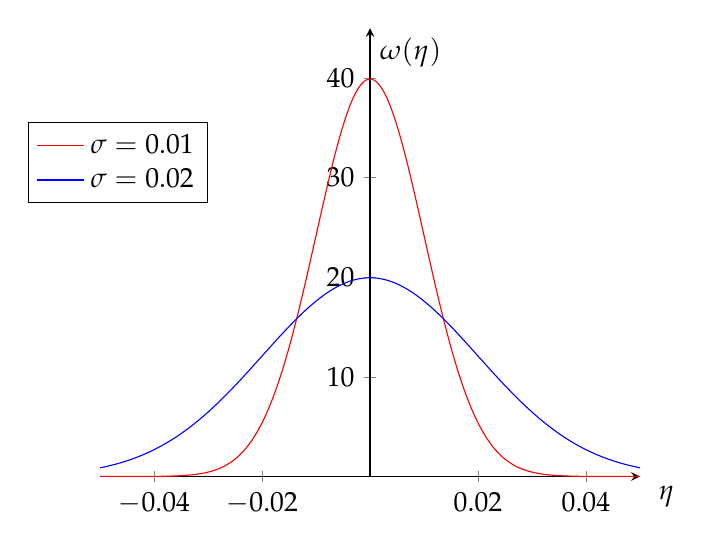
\begin{tikzpicture}
    \begin{axis}[
    axis lines = center,
    ymin=0, ymax=45,
    xlabel = $\eta$,
    scaled x ticks = false,
    % x tick label style={},
    x label style={at={(axis description cs:1.05,0.0)},anchor=north},{/pgf/number format/fixed},
    ylabel = $\omega(\eta)$,
    legend style={at={(0.2,0.7)},anchor=east},
    legend cell align=left,
    ]
    \addplot [
    domain=-0.05:0.05, 
    color=red,
    samples=200,
    ]
    { 1/(sqrt(2*pi)*0.01)*exp(-x^2/(2*0.01^2))};
    \addplot [
    domain=-0.05:0.05, 
    color=blue,
    samples=200,
    ]
    { 1/(sqrt(2*pi)*2*0.01)*exp(-x^2/(2*(2*0.01)^2))};
    \addlegendentry{$\sigma=0.01$}
    \addlegendentry{$\sigma=0.02$}
    \end{axis}

  \end{tikzpicture}
    \caption[Normal Distribution: Used as a weight function]{Using the probability density function of the normal distribution to 
    calculate the score of a point in order to have a well defined maximum if a point lies directly on the circle and $\eta(r) = 0$. 
    Increasing the $\sigma$ increases the width of the function and by extension increases the score of points who are not lying 
    directly on the circle}
  \label{fig:gauss}
\end{figure}
Equation \ref{eq:weight_function} is of course just the circle equation with $c_x, c_y$ being the known coordinates of the center of 
the circle, $x, y$ are the data points and $r$ is the radius. If a lot of the data points have the same distance $r$ from the circle 
center there will be a high score for this particular radius. The index for the highest score can then be used to find the 
corresponding radius. The pseudo code for this Hough transform is shown in Code Snippet \ref{pc:1dHT}. An example of a resulting radius
histogram is shown in figure \ref{fig:1d_ht_radius_score}

\begin{codesnippet}[htb]
  \begin{lstlisting}
  DMENSION = 1001
  r= linspace(0,1,DIMENSION)
  for c_x, c_y in centers:
    scores = zeros(DIMENSION)
    for x,y in allPoints:
      s = 2*BIN_WIDTH
      eta = (c_x-x)**2 + (c_y-y)**2 - r**2
      scores += 1. / ( sqrt( 2 * Pi ) * s ) 
                 * exp( -( eta ** 2 ) 
                  / ( 2 * s ** 2 ) )
    index = max(scores)
    circle = {}
    circle['center'] = c
    circle['radius'] = r[index]
\end{lstlisting}
\caption[Pseudo Code 1D HT]{Pseudo code for the 1D Hough transform. r is an array of length 1001 so $\eta$ will also be an 
array of length 1001. Scores is where the score for each iteration is stored. For each point the score is computed and added 
to the scores array and at the end the index with the highest score is the index we need to get the radius}\label{pc:1dHT}
\end{codesnippet}

\begin{figure}[tb]
  \centering
  \includegraphics[width=0.8\textwidth]{sim_pics/1D_HT/radius_scores_5_circles_30_bg_1}
  \caption[Graph visualisation of a 1D radius histogram]{A graph visualisation of a 1D radius histogram. The peak between $0.2$ 
  and $0.3$ has by far the highest score and the bin
  position of the peak is the radius candidate for a given circle center ($c_x, c_y$)}
  \label{fig:1d_ht_radius_score}
\end{figure}

\subsubsection{Complexity} % (fold)
The complexity of this algorithm is of $\mathcal{O}(n)$ where $n$ is the number of bins in the radius histogram.
\label{ssub:complexity_1d}

% subsubsection complexity (end)

% subsection 1d_known_center_find_radius (end)
\subsection{2D: Known radius - find center} % (fold)
\label{sub:2d_known_radius_find_center}
In this case the radius is known and the $x$ and $y$ coordinates of the center $(c_x, c_y)$ are unknown. Now, the accumulator is 2 
dimensional. The range of that space is the dimension of the detection plane which for this thesis is $[-0.5,0.5]$. The size of the 
bins is chosen to be 0.001 since the known radius given from the test data was of the same order. So if the detection plane was in 
reality 1\,m by 1\,m the binning of the accumulator in each dimension is 1 mm. As in the one dimensional case we use the scoring function 
\ref{eq:score_function} in combination with the weight function \ref{eq:weight_function}.
Since it is likely that two circles have the same radius a mechanism has to be introduced the remove points from the data set that
have been used for a ring. If two circles have the same radius the algorithm would only ever find the one with the higher score. To avoid
this once a circle has been found a check for each data point is made to see whether or not it lies on the circle and if yes is removed.

\begin{codesnippet}[htb]
\begin{lstlisting}
  DIMENSION = 1001
  xbins = linspace(-0.5,0.5,DIMENSION)
  ybins = linspace(-0.5,0.5,DIMENSION)
  x, y = broadcast_arrays( xbins[..., newaxis], 
                           ybins[newaxis,...] )

  for r in Radiuses:
    weights = zeros( (DIMENSION,DIMENSION) )
    for xd,yd in allPoints:
      s = 2*BIN_WIDTH
      eta = (xd-x)**2 + (yd-y)**2 - r**2      
      weights += 1. / ( sqrt( 2 * pi ) * s ) 
                 * exp( -( eta ** 2 ) 
                 / ( 2 * s ** 2 ) )
    i, j = argmax(weights)
    removeUsedPoints()
    circle['Center'] = (xbins[i], ybins[j])
    circle['Radius'] = r
\end{lstlisting}
  \caption[Pseudo code 2D HT]{Pseudo code for the 2D Hough transform. \texttt{xbins} and \texttt{ybins} are arrays of length 1001. Here we use array 
  broadcasting in order to avoid for loops and the weights can be evaluated in one line. This means that the x and y variables have 
  dimension (1001,1001) but they don't take up that much memory. The x variable for example just broadcasts its value from the first 
  row down to all the other rows and for y it broadcasts the first column to all the other columns. The variable weights is a 1001 by 
  1001 matrix. Again the entry with the highest score is the candidate for a possible circle center and if found is stored in a final 
  variable called circle.}
\end{codesnippet}


\subsubsection{Complexity} % (fold)
\label{ssub:complexity_2d}
The complexity of this algorithm is $\mathcal{O}(n\times m)$ where $n$ and $m$ are the number of bins per coordinate respectively per 
the histogram. The calculation of the weight has to be done for each data point of the 2D histogram. So in a $1000\times 1000$ histogram 
with 400 data points we calculate 400'000'000 times the weight of a grid point. Reducing the dimensions of the histogram weakens the 
accuracy of the whole algorithm but can speed up the calculations considerably. With a $1000\times 1000$ histogram the resolution in each 
space dimension is $1$\,mm. The RICH Technical Design Report states the resolution of the HPD is $2.5$\,mm $\times$ $2.5$\,mm.

The need (not entirely true -- see below) to calculate the weight for each grid point and data point means that there is a loop over 
data points and two loops for the $x$ and $y$ coordinate of the grid. To improve upon that there is the possibility of array broadcasting.
% subsubsection complexity (end)

\newpage
\subsubsection{Array broadcasting}
Consider following one dimensional arrays where $x$ is a 1D histogram binning entries from 1 to 4 and same for $y$. 
\begin{align*}
  x &= [1, 2, 3, 4]\\
  y &= [1, 2, 3, 4]  
\end{align*}
Now all combinations between an element of $x$ and $y$ represent a 2D grid $\left((1,1), (1,2), ...\right)$. So to iterate through all those grid points one would have to create 2 for-loops iterating through $x$ and $y$ as shown in below pseudo code snippet: %\ref{pc:nested_loops}.
% \begin{figure}[tb]
    \begin{lstlisting}
  def noBroadcast():
  a = np.random.randn(100)
  b = np.random.randn(100) 
  for x in a:
    for y in b:
      print (1-x)^2 + (2-y)^2 - 9
\end{lstlisting} 
% \caption[2 for-loops example]{To calculate the statement for every value in $a$ and $b$ the program has to do nested for-loops}\label{pc:nested_loops}
% \end{figure}

This is not only slow but also doesn't look too nice if there are even more loops.
Broadcasting now turns the one dimensional arrays of length $n$ into two $n\text{ by }n$ matrices
\[
  x = \begin{bmatrix}
  1 & 1 & 1 & 1 \\
  2 & 2 & 2 & 2 \\
  3 & 3 & 3 & 3\\
  4 & 4 & 4 & 4
  \end{bmatrix}
\]
and
\[
  y = \begin{bmatrix}
  1 & 2 & 3 & 4 \\
  1 & 2 & 3 & 4 \\
  1 & 2 & 3 & 4 \\
  1 & 2 & 3 & 4 
\end{bmatrix}
\]
\noindent\begin{minipage}{\linewidth}
And with this the loops can be omitted:
\begin{lstlisting}
def withBroadcast():
  a = np.random.randn(100)
  b = np.random.randn(100) 
  x,y = np.broadcast_arrays(a[...,np.newaxis],
                            b[np.newaxis,...])
  print (1-x)^2 + (2-y)^2 - 9
\end{lstlisting}  
\end{minipage}
In this case this prints a $4$ by $4$ array with the function evualted for each combination of entries of $x$ and $y$
\[
  \begin{bmatrix}
    -8& -9& -8& -5\\
    -7& -8& -7& -4\\
    -4& -5& -4& -1\\
     1&  0&  1&  4
       \end{bmatrix}
\]
%
\begin{minipage}{\linewidth}
A runtime comparison shows   
\begin{lstlisting}
In [3]: %timeit withBroadcast()
10000 loops, best of 3: 76.8 us per loop

In [4]: %timeit noBroadcast()
100 loops, best of 3: 7.99 ms per loop
\end{lstlisting}
So the version with broadcasting is 100 times faster than the double loop. And the memory consumption is moderate since the 
broadcasted entries aren't new memory locations but just refer to the initial array.
\end{minipage}


\subsubsection{Optimizations} % (fold)
\label{ssub:optimizations}
It was mentioned before that for each data point the weight for the whole grid has to be calculated. This is not true. In the 2D case 
each grid point is a potential center for a circle only if it is not further a away and a threshold radius $R_T$, so if a grid point is 
further away than this threshold radius this calculation could be skipped. This could probably be done even smarter with the use of a 
sub grid so only points in the surrounding sub grids are considered of being possible centers and not the whole grid.

% subsubsection optimizations (end)

\subsubsection{Simple example: 2 circles without background} % (fold)
\label{ssub:simple_example_of_2_circles_without_background}
\begin{figure}[hp]
  \centering
  \includegraphics[width=0.5\linewidth]{sim_pics/2D_HT/center_scores_2_circles_0_bg_1}%
  \includegraphics[width=0.5\linewidth]{sim_pics/2D_HT/center_scores_2_circles_0_bg_2}

  \caption[2D weight matrix, first iteration]{(Left) 2D weight matrix in the first iteration of the Hough transform algorithm. (Right) Second iteration
  of the 2D weight matrix of the Hough transform. Points that satisfied the condition being less than a certain $\epsilon$ away from the radius found in the first iteration are removed leaving (hopefully) only points available that belong to the second circles}
  \label{fig:2d_weights_01}
\end{figure}
% subsubsection simple_example_of_2_circles_without_noise (end)
% section 2d_known_radius_find_center (end)

\subsection{3D: All parameters unknown} % (fold)
\label{sub:3d_nothing_is_known_find_everything}
In this case all that is known are the data points and the algorithm has to retrieve both the center and the radius of the circles. 
The accumulator space is now three dimensional, two for the coordinates of the center and one for the radius. Similar to the 2D case, 
array broadcasting (see code snippet~\ref{pc:3D_broadcasting}) is used to speed up the calculations of the weights. Furthermore, 
the algorithm has to decide itself whether or not  all circles have been found since there unlike in the previous two cases, there isn't 
any information availabe about the circles so a condition has to be set to decide when there are no more circles.

For deciding whether or not the algorithm has found all rings, a simple score threshold is used that whenever the highest score
of the weight matrix is less than the threshold the algorithm stops and it is assumed that all circles have been found. The threshold
used in this thesis has been determined by trial and error and was set to a score of $3500$. The pseudo code for calculating the weights 
and the threshold check is shown in \ref{pc:3D_threshold}. As in the 2D Hough transform in the 3D case the algorithm has to remove data 
points that have contributed to the highest score. If not done the algorithm will loop endlessly because always the same score will be 
found. Once the highest score has been found the center coordinates and radius are extracted from the histogram and with these the 
algorithm calculates for every data point, if this data point lies on that circle given the extracted center and radius.If the data point 
lies within two times the bin width of the circle, it will be removed (see \ref{pc:remove_points}).

\begin{codesnippet}[htbp]
  \begin{lstlisting}
xbins = np.linspace(-0.5,0.5,DIMENSION)
ybins = np.linspace(-0.5,0.5,DIMENSION)
rbins = np.linspace(0,0.5, R_DIMENSION)

x,y,r = np.broadcast_arrays(\
            xbins[np.newaxis,...,np.newaxis],\
            ybins[np.newaxis,np.newaxis,...],\
            rbins[...,np.newaxis,np.newaxis])
\end{lstlisting}
\caption[3D broadcasting]{Broadcasting of the 3 arrays $x,y,r$. With this 3 for-loops can be avoided improving speed and readability
of the code.}
\label{pc:3D_broadcasting}
\end{codesnippet}

\begin{codesnippet}[htbp]
  \begin{lstlisting}
while True:
  weights = np.zeros(\
         (R_DIMENSION, DIMENSION, DIMENSION))

  for x0,y0 in data['allPoints']:
    s = 0.001
    eta = (x-x0)**2 + (y-y0)**2 - r**2
    weights += 1./( sqrt( 2 * sconst.pi ) * s )*\
                      np.exp( -( eta ** 2 ) / \
                      ( 2 * s ** 2 ) )
  index = np.argmax( weights )
  rr,ii,jj = np.unravel_index( index, 
              (R_DIMENSION, DIMENSION, DIMENSION))
  score = weights[rr][ii][jj]
  if score < THRESHOLD:
    break  
\end{lstlisting}
\caption[Calculation of weights and threshold check for 3D HT]{The while loop works as long as the found score is higher than
\texttt{THRESHOLD}. If the score is lower than the threshold the loop breaks and the function returns the results that have been found.}
\label{pc:3D_threshold}
\end{codesnippet}

As before a scoring function is used but this time the scoring function is of the form $\eta(x,y,r)$ and each point in weights then stands
for the score of the $x,y,r$ entries and their respective value.
\begin{equation}
  \eta(x,y,r) = (x - d_x)^2 + (y - d_y) - r ^ 2
\end{equation}
where $d_x$ and $d_y$ are the data points.
\begin{equation}
  w(\eta) = \frac{1}{\sqrt{2\pi}\sigma}\exp\left( \frac{-\eta^2}{2\sigma^2}\right)
\end{equation}

\begin{codesnippet}[htbp]
\begin{lstlisting}
circle['center'] = (xbins[ii], ybins[jj])
circle['radius'] = rbins[rr]
circles.append(circle)

used_xy += [tup for tup in data['allPoints'] if
    abs( ( tup[0] - circle['center'][0] ) ** 2 +
         ( tup[1] - circle['center'][1] ) ** 2 -
         circle['radius'] ** 2 ) < 2 * 0.001]
data['allPoints'][:] = 
            [tup for tup in data['allPoints'] if 
    abs( ( tup[0] - circle['center'][0] ) ** 2 + 
         ( tup[1] - circle['center'][1] ) ** 2 - 
         circle['radius'] ** 2 ) >= 2 * 0.001]  
\end{lstlisting}
\caption[Remove used points]{In order to avoid finding the same ring over and over again the algorithm has to remove points that
belong to a ring. If a data point lies within two times the bin width of a ring the algorithm considers that data point to be 
part of that circle and removes that data point from the list.}
\label{pc:remove_points}
\end{codesnippet}

\subsubsection{Complexity} % (fold)
\label{ssub:complexity}
The complexity of this algorithm is of order $\mathcal{O}(m\times n\times r)$. As in the case the 1D and 2D Hough transform the accuracy
directly depends on the binning. For the 3D Hough transform to match the resolution of the HPD of the LHC\textit{b} RICH detector a binning 
of 400 makes sense if the detector dimensions are $1$\,m$\times1$\,m.
% subsubsection complexity (end)

\subsubsection{Optimisations} % (fold)
\label{ssub:optimisations}
As for the 2D HT introducing a sub grid can be introduced for the $x,y$ plane so only grid points in the vicinity of a data point are used
for calculating the score.
% subsubsection optimisations (end)
% subsection 3d_nothing_is_known_find_everything (end)

\section{Combinatorial triplet Hough transform}
\label{sec:combinatorial_approach}
A circle is uniquely defined by 3 points and its radius and center can be calculated from the coordinates of these points. If there are 
15 points lying on the same circle there are 455 possible combinations of triplets According to the binomial distribution.
\[
   \binom{N}{3} = \frac{N!}{k!(N-k)!}
 \] 
Calculating the center and radius for these 455 triplets should result in the same center ($x,y$) and same radius $r$ for all the triplets 
(floating point inaccuracy not considered). 

Having one random background hit in addition to the 15 circle hits increases the number of triplets number to 560. The triplets with points solely consisting of points on the circle still have the same center and radius but the new combinations that now include a background hit will vary and it is unlikely that any two triplets that include the background point will have the same center and radius. Here is an overview of the algorithm studied in this thesis.

\begin{enumerate}
\item Build all possible triples of points given the data points
\item For all triplets calculate the center and the radius of the potential circle
\item Remove all triplets that yield a radius bigger than a certain threshold.
\item Create a histogram with the distribution of $r$ for the remaining triplets. Peaks in this histogram hint to a circle.
\item Scan the radius histogram for peaks and look at the 2D histogram of ($x,y$) for the triplets belonging to a given peak in the $r$ distribution. If there is also a peak in the ($x,y$) histogram the set of the points of the triplets lie on a circle with a radius and center given by the peaks in the $r$
and ($x,y$) histograms.
\end{enumerate}

\subsection{Generating the triplets} % (fold)
\label{sub:generating_the_triples}
To generate the triplets the built-in function \texttt{itertools.combinations()} of python is used. The input is an iterable, in our case a
list of tuples (each tuple is the $x$ and $y$ coordinate of a data point) which is used to create all possible combinations of triples (of said tuples).

% subsection generating_the_triples (end)

\subsection{Calculating the Circle given 3 points}

Let $(A,B,C)$ be a triplet of points in a 2D plane and $a,b,c$ the lengths of the sides opposite to the respective corner.
%
The semiperimeter is defined as
%
\begin{equation}
  s = \frac{a+b+c}{2}.
\end{equation}
%
Using this we can calculate the radius $R$ of the circumcircle of the triangle $\overline{ABC}$:
\begin{equation}
  R = \frac{abc}{4\sqrt{s(a+b-s)(a+c-s)(b+c-s)}}
\end{equation}
We have $\lambda_1, \lambda_2, \lambda_3$ as the barycenteric coordinates of the circumcenter:
\begin{align}
  \lambda_1 &= a^2\cdot(b^2+c^2-a^2)\\
  \lambda_2 &= b^2\cdot(a^2+c^2-b^2)\\
  \lambda_3 &= c^2\cdot(a^2+b^2-c^2)
\end{align}
Multiplying a matrix consisting of the column vectors of $A,B,C$ with a column vector of $\lambda_1, \lambda_2, \lambda_3$ and dividing the resulting vector by the sum of the barycentric coordinates (for normalization) yields the coordinate of the circumcenter of the triangle $\overline{ABC}$ 
%
\begin{equation}
  \begin{pmatrix}
    A_x & B_x & C_x \\
    A_y & B_y & C_y
  \end{pmatrix} \cdot \begin{pmatrix}
    \lambda_1\\
    \lambda_2\\
    \lambda_3
  \end{pmatrix} = \boldsymbol{P'}
\end{equation}
%
\begin{equation}
  \frac{\boldsymbol{P'}}{\lambda_1+\lambda_2+\lambda_3} = \boldsymbol{P}
\end{equation}
%
\begin{figure}[tb]
\centering
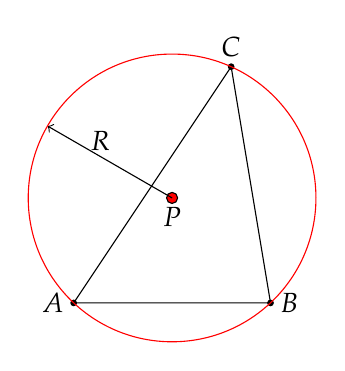
\begin{tikzpicture}
\coordinate (A) at (0,0);
\coordinate (B) at (2.5,0);
\coordinate (C) at (2,3);
\coordinate (Ci) at (1.25,1.33333);
\def\r{1.827}
\draw[thin] (A) -- (B) -- (C) -- cycle;
\node[left] at (A) {$A$};
\node[right] at (B) {$B$};
\node[above] at (C) {$C$};
\node[below] at (0.34,2.3) {$R$};
\draw[fill=black] (A) circle (1pt);
\draw[fill=black] (B) circle (1pt);
\draw[fill=black] (C) circle (1pt);
\draw[fill=red] (Ci) circle (2pt) node [below] (Ci) {$P$};

\draw[->] (1.25,1.33333) -- +(150:1.827);
\draw[red] (1.25,1.33333) circle (1.827);
\end{tikzpicture}
\caption{The circumradius ($R$) and the circumcenter ($P$) of a circle defined by three points ($A,B,C$).}
\label{fig:circum_fig}
\end{figure}



\subsection{Finding the radius and center of a circle} % (fold)
\label{sub:finding_the_radius_and_center_of_a_circle}
Once $R$ and $\mathbf{P}$ are known these values are stored as a pair in a tuple. A list holds then all tuples of ($R, \mathbf{P}$) values
for all the triplets.

The next step is binning this data for $R$. This is done in a way that the center data of a tuple is associated with the $R$ bin of the tuple.
This allows the algorithm when looking for a peak in the $R$ histogram to access the center data for this $R$ value. Essentially it
splits the problem first in a 1D Hough transform where the algorithm looks for a peak in the radius distribution and with a given radius
the algorithm can then search the ($x,y$) space for a peak and thus determine the center.

\subsubsection{Ring finding threshold} % (fold)
\label{sub:different_thresholds}
The algorithm applies a very simple threshold to decide whether a candidate is a ring or not. Assume just one ring with 10 points. With
these 10 points the algorithm creates 120 triplets $\left(\binom{10}{3}\right)$. For each of these triplets the radius and the ring are calculated.
Since they all belong to the same ring the radius histogram has one peak at the ring radius and the center histogram has 1 peak at
the ring center. If the threshold is now smaller than 120 then this ring will be found and otherwise ignored. So essentially we can 
decide how many points per ring are needed in order to be recognized as ring. This puts a requriement on the minimum number of points
a ring should have and the threshold is
\[
  \binom{\text{Number of Points}}{3} = \text{Threshold}
\]

\subsubsection{Finding the radius} % (fold)
\label{ssub:finding_the_radius}
Once the radius histogram is created the algorithm looks for the index where the maximum value of the histogram is stored. The algorithm
checks first if the sum of the entry at the index and the left and right neighbour exceeds the radius threshold which is a tuning parameter.
If the value exceeds the threshold the algorithm extracts the center data from the index and its left and right neighbour respectively.

\subsubsection{Finding the center} % (fold)
\label{ssub:finding_the_center}
Having a list of ($x,y$) points and one radius the algorithm now looks for a peak in the ($x,y$) plane. Similar as the for radius also
the directly adjacent neighbour bins are added to the sum. If the sum exceeds the center threshold then radius and the center coordinates are 
saved as a circle candidate.
% subsubsection finding_the_center (end)
% subsubsection finding_the_radius (end)
% subsection finding_the_radius_and_center_of_a_circle (end)


\subsection{Combinatorics}
	

The main drawback of this method is that the combinatorics increase with for high number $N$ of data points as \( \binom{N}{3} \). 
For example, for 200 data points the number of triplets is

\[ \binom{200}{3} = 1'313'400 \]
and for 300 data points it is
\[ \binom{300}{3} = 4'455'100. \]

The execution time of the algorithm is roughly of the order of $\mathcal{O}(N^3)$ which can be easily seen when taking the upper bound of $\binom{N}{3} \leq \frac{N^3}{3!}$ (see figure \ref{fig:binom_growth}). 
\begin{figure}[ht]
\centering
  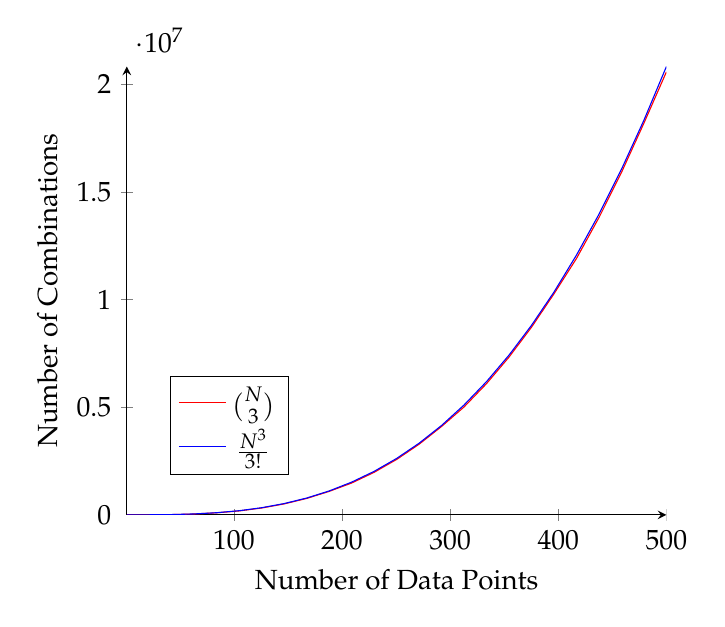
\begin{tikzpicture}
    \begin{axis}[
    axis lines = left,
    xlabel = Number of Data Points,
    ylabel = {Number of Combinations},
    legend style={at={(0.3,0.2)},anchor=east},
    ]
    \addplot [
    domain=1:500, 
    color=red,
    ]
    { factorial(x)/(factorial(x-3)*factorial(3))};
    \addplot [
    domain=1:500, 
    color=blue,
    ]
    { x^3/factorial(3)};
    \addlegendentry{$\binom{N}{3}$}
    \addlegendentry{$\frac{N^3}{3!}$}
    \end{axis}

  \end{tikzpicture}
    \caption[Complexity of the combinatorial triplet Hough transform]{Scaling of the algorithm. Binomial Growth with $\binom{N}{3}$ compared with the approximation $\frac{N^3}{3!}$ where $N$ is the number of data points. So the algorithm runs in the order of $\mathcal{O}(N^3)$}
  \label{fig:binom_growth}
\end{figure}


\subsubsection{Optimisation} % (fold)
\label{ssub:improvement_of_speed}

The algorithm needs a threshold on the minimum height of the peak in the ($x,y$) and $r$ histograms in order to decide if a candidate is a circle or not. The threshold is defined as such that the minimum number of points on a circle has to be $\binom{T}{3}$ in order to be considered as a circle candidate. 

But not only the number of triplets generated is a speed bump for the execution time but also the time it takes to create the triplets scales with $\frac{N^3}{3!}$. If there was a way to reduce not only the number of triplets created but also the time needed to create them would speed up the algorithm considerably.

This leads to the following idea: to split the original data set randomly into two lists. For each of these lists all possible combinations 
of triplets is generated separately and the two lists are then merged in one single list. In Figure~\ref{fig:binom_half_growth} 
the difference in combinatorics between $\binom{N}{3}$ and $2\binom{\frac{N}{2}}{3}$ can be seen.

\begin{figure}[b]
\centering
  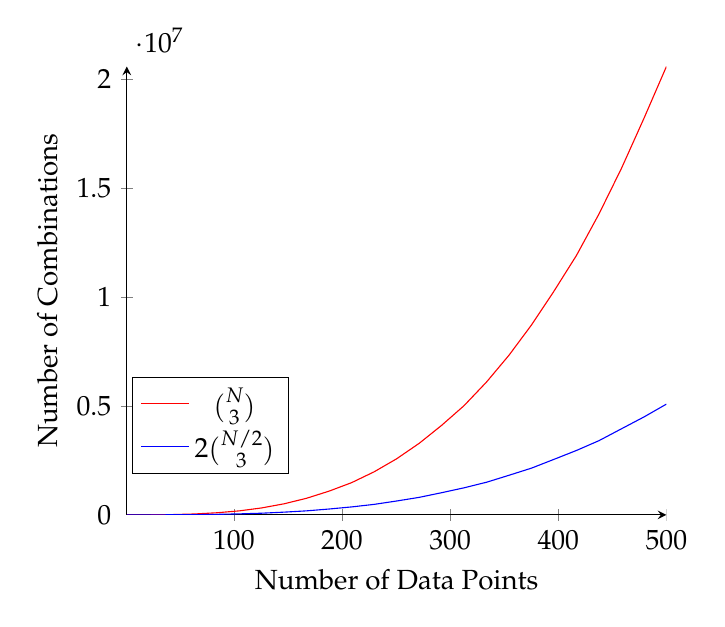
\begin{tikzpicture}
    \begin{axis} [
      axis lines = left,
      xlabel = Number of Data Points,
      ylabel = {Number of Combinations},
      legend style={at={(0.3,0.2)},anchor=east},
    ]
    \addplot [
    domain=1:500, 
    color=red,
    ]
    { factorial(x)/(factorial(x-3)*factorial(3))};
    \addplot [
    domain=1:500, 
    color=blue,
    ]
    { 2*factorial(x/2)/(factorial(x/2-3)*factorial(3)) };
        \addlegendentry{$\binom{N}{3}$}
    \addlegendentry{$2\binom{N/2}{3}$}
    \end{axis}
  \end{tikzpicture}
  \caption{Number of combinations with $\binom{N}{3}$ compared to the number of combinations generated from $\binom{N/2}{3}$}
  \label{fig:binom_half_growth}
\end{figure}

The problem with this approach is the possible loss of information and efficiency, since the
algorithm has a threshold that defines how many entries a bin in the ($x,y$) and $r$ histograms must 
have in order to be accepted as a candidate circle.
This threshold should be high enough that triplets that contain noise points
do not contribute significantly to the circle candidates but low enough that real circles with a
low number of points can still be found.

%assume 10 points is threshold - expand on that
So the question is what is probability of splitting points that belong to a specific circle in such way that at least one list
has enough points that their combinations can reach the threshold.

In Figure~\ref{fig:ratios} it can be seen that even if we split the lists there is a more 
than 50\% chance that we lose no information once a circle has 13 points.
\begin{figure}[htb]
  \centering
  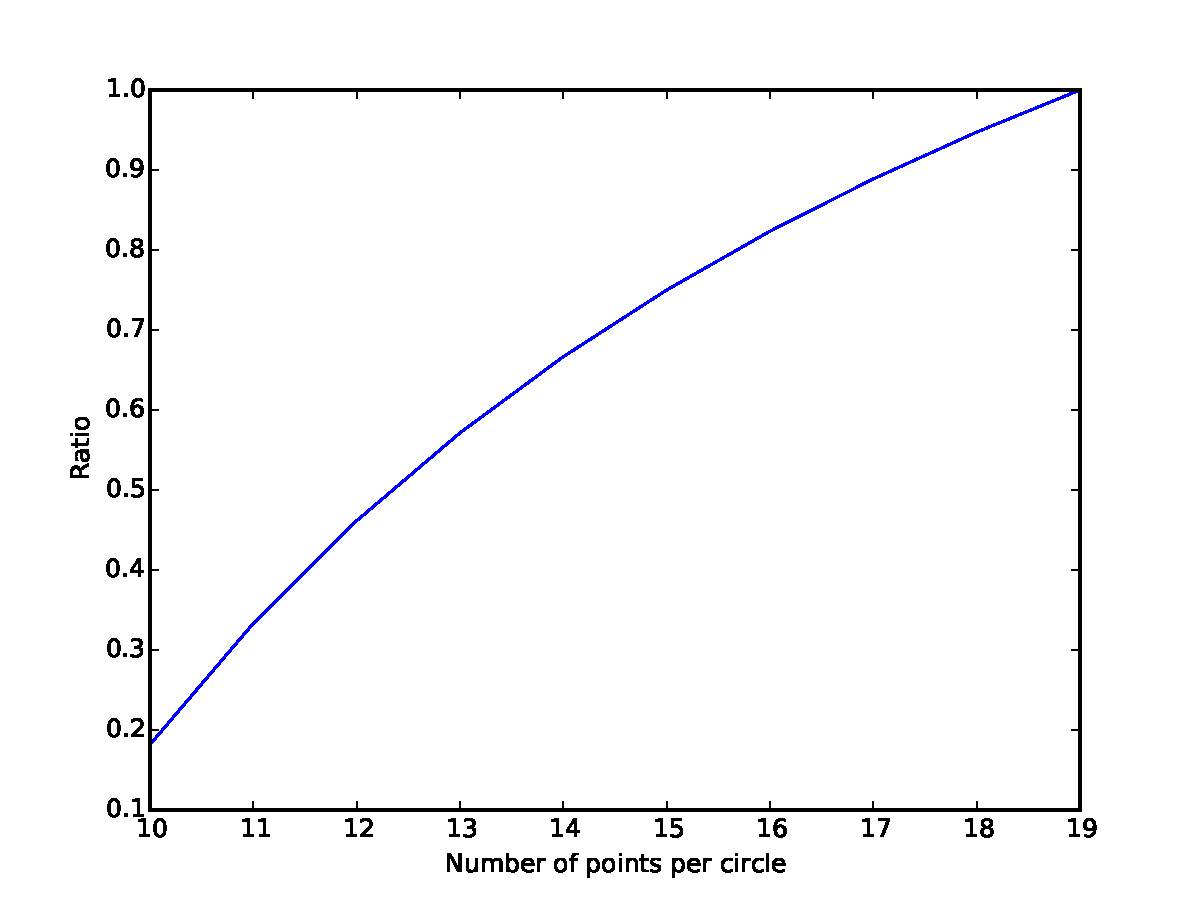
\includegraphics[width=\textwidth]{pics/ratio.pdf}
  \caption{The probability when splitting randomly a list of $x$ points into two that one list has more than 10 points.}
  \label{fig:ratios}
\end{figure}

\subsubsection{Bin size dependency} % (fold)
\label{ssub:bin_size_dependency}
In the conventional Hough transform the weight function is calculated with the
bin centers of the accumlator space as variables. The larger the binning of the accumulator is, the less accurate the calculations become. 
The number of bins is the main factor for the execution time of the algorithm. The advantage of this combinatorial approach lies in the 
fact that the parameters can be caculated accurately up to floating point precision and a histogram is only needed group the results. 
A fine binning only marginally affects the execution time of the algorithm since the only operation done in the histogram is finding the 
maximas and this is only done a few times (stops when the found maximum is lower than the ring finding threshold).
% subsubsection bin_size_dependency (end)

% subsubsection optimisation (end)

\subsection{Possible optimisation: average radius of random circles in a unit square} % (fold)
\label{ssub:average_radius_of_random_circles_in_a_unit_square}
An interesting property of calculating the radius of triplets generated from points that are distributed uniformely in the unit square is 
that they always obey a certain shape.

To prove this the expected area of a triangle formed by three points randomly chosen from the unit square\footnote{This proof is taken
from \cite{Blatter:2015}} has to be calculated. Let \( A = (x_A, y_A),\ B = (x_B, y_B),\ C = (x_C, y_C)\) be the vertices of the random triangle \( T \). We consider the case where \( y_A
> y_B > y_C \) which takes $\frac{1}{6}$ of the total ``Volume''. Fix \( y_A, y_B, y_C \) for the moment and we can write.
\[
  y_B = (1-t)y_A + ty_C, \qquad 0 \leq t \leq 1.
\]
The side $AC$ of $T$ intersects the horizontal level $y=y_B$ at the point $S=(s,y_B)$ with
\begin{equation}
  s = s(x_A,x_C,t) = (1-t)x_A + tx_C
\end{equation}
The area $X$ of $T$ is then given by
\[
  X = \frac{1}{2}\lvert x_B - s\rvert(y_C - y_A)
\]
We now start integrating with respect to our six variables. The innermost integral is with respect to $x_B$ and gives

\begin{align}
  X_1 &:= \int_0^1X\text{d}x_B=\frac{1}{2}(y_C-y_A)\left( \int_0^s(s-x_B)dx_B + \int_s^1(x_B-s)dx_B\right)\nonumber\\
      &\phantom{:}= \frac{1}{4}(y_C-y_A)(1+2s+2s^2)\nonumber
\end{align}
Next we integrate over $y_B$:
\begin{align}
  X_2 &:= \frac{1}{4}\int_0^1\int_{y_A}^1(y_C-y_A)^2\,dy_C\,dy_A\,\times\,\int_0^1\int_0^1\int_0^1(1-2s+2s^2)\,dt\,dx_C\,dx_A  \nonumber
\end{align}
This gives
\[
  X_3 = \frac{1}{4}\cdot \frac{1}{12} \cdot \frac{11}{18} = \frac{11}{6\cdot144}
\]
But generalizing our assumption at the beginning $y_A < y_B < y_C$ we multiply this result by $6$ and obtain then $\frac{11}{144}$.

From \cite{Weisstein2016} follows that the average area of a triangle in a unit circle is $\frac{3}{2\pi}$ so dividing this area by the
area of the unit circle gives the expected area covered by a triangle in an arbitrary circle

\[
\frac{\text{Expected area of a triangle in a unit circle}}{\text{Area of the unit circle}} = \underbrace{\frac{\frac{3}{2\pi}}{\pi r^2}}_{r=1} = \frac{3}{2\pi^2}
\]

So finally the average area of a random circle can be obtained by dividing the average area of a triangle from the unit square by expected
area covered by a triangle in an arbitrary circle so essentially the average area of a random circle within the unit square:

\[
  \frac{\frac{11}{144}}{\frac{3}{2\pi^2}} = \frac{11\pi^2}{216}
\]

This should be equal to $\pi R^2$ where $R$ is the average radius of a random circle in the unit cube

\begin{align}
  R\pi^2 &= \frac{11\pi^2}{216}\nonumber\\
  R &= \sqrt{\frac{11\pi}{216}} = 0.399986\nonumber
\end{align}

Generating a random background and then plotting the radius histogram for this data set shows that there is indeed a peak around
 $R\approx 0.4$.

 \begin{figure}[tb]
   \centering
   \includegraphics[width=0.8\textwidth]{sim_pics/background_radius_for_diff_background}
   \caption[Radius distribution for background]{Radius distribution for uniformly generated 
    background. The expected value of $R\approx 0.4$
   is quite well represented for differently sized data sets}
   \label{fig:rad_dist}
 \end{figure}

% subsubsection average_radius_of_random_circles_in_a_unit_square (end)
% chapter methods (end)
\chapter{Results}
\label{cha:results}
In this section results for the conventional 1D, 2D, 3D Hough transform and 
the combinatorial triplet Hough transform are presented. 1D, 2D and 3D Hough transform
were not pursued in depth. They are presented here as they offer a 
way of understanding how each extra dimension expands the algorithm and also
shows the flaws with each added dimension.

For the 1D, 2D and 3D Hough transform very simple data was used. There were 
no physical constraints when generating the circles and the number of points
per circle and the distribution of the radiuses doesn't reflect the real data obtained
by LHC\textit{b}.

For these conventional Hough transforms following data sets were tested

\begin{itemize}
  \item 1 circle and 600 background hits
  \item 2 circles and 0 background hits
  \item 5 circles and 30 background hits
  \item 6 circles and 200 background hits (results only shown for 2D and 3D)
\end{itemize}


The points per circle ranges from 17--31 in all the circles from the data sets
and the background is uniformly distributed in the unit square. The event with 1
circle and 600 background hits is meant to test how robust the algorithm is with a 
lot of background hits. The second test case is meant to test if the algorithm can handle
two circle objects, the third is a mix between several circles and background and the last
event is a special case where two circles lie very close to each other and for the 2D
and 3D case where the center is unknown these algorithms can encounter problems with
detecting the right circles. In Figure~\ref{fig:real_ht_results}
the real circles plotted from simulation parameters for the different events.

\begin{figure}
\centering
        \subfloat[][1 circle, 600 background hits.]{\includegraphics[width=0.5\textwidth]{sim_pics/1D_HT/real_result_1_circle_600_bg}}
                \label{fig:real_1c600bg}%
        \subfloat[][2 circles, 0 background hits]{\includegraphics[width=0.5\textwidth]{sim_pics/1D_HT/real_result_2_circles_0_bg}}
                \label{fig:real_2c0bg}

        \subfloat[][5 circles, 30 background hits]{\includegraphics[width=0.5\textwidth]{sim_pics/1D_HT/real_result_5_circles_30_bg}}
                \label{fig:real_5c30bg}%
        \subfloat[][6 circles, 200 background hits]{\includegraphics[width=0.5\textwidth]{sim_pics/2D_HT/real_result_6_circles_200_bg}}
                \label{fig:real_6c_200bg}%
        \caption{These are the circles as generated by the simulation.\label{fig:real_ht_results}}
\end{figure}

\section{1D Hough transform results} % (fold)
\label{sec:1d_hough_transform_results}

There are two different plots: for each set the radius score is shown in Figures~\ref{fig:1d_ht_radius} and \ref{fig:1_2_c_radius} and the resulting
circles in Figure~\ref{fig:1d_ht_results}. The radius score is a 1D plot of the weight function 
$w(\eta)$~\ref{eq:weight_function}. The highest peak indicating the maximum score and its location telling the value of the radius.
The resulting circle plot is the center (which was known) and the extracted radius combined, drawing the resulting circle. 
The numerical values from the high scores and the second highest score are shown in Table~\ref{tab:1d_scores}. 
The algorithm has no problems to find any of  the circles even with background. But this was expected as the 
algorithm only needs to search in one dimension and makes the whole process very easy. The fourth event was also tested for the 1D Hough
transform but not shown in this thesis because they didn't add anything that is not already covered with the first 3 events.

% subsection overview_of_the_results (end)
\begin{figure}[htp]
        \centering
        \subfloat[][1 circle, 600 background hits. \label{fig:1c600bg}]{\includegraphics[width=0.3\textwidth]{sim_pics/1D_HT/result_1_circle_600_bg}}
        ~ %add desired spacing between images, e. g. ~, \quad, \qquad etc.
          %(or a blank line to force the subfigure onto a new line)
       \subfloat[][2 circles, 0 background hits]{\includegraphics[width=0.3\textwidth]{sim_pics/1D_HT/result_2_circles_0_bg}}
                \label{fig:2c0bg}
        ~ %add desired spacing between images, e. g. ~, \quad, \qquad etc.
          %(or a blank line to force the subfigure onto a new line)
        \subfloat[][5 circles, 30 background hits]{\includegraphics[width=0.3\textwidth]{sim_pics/1D_HT/result_5_circles_30_bg}}
                \label{fig:5c30bg}
        \caption{Circles found by the 1D Hough transform. The circle in Figure~\ref{fig:1c600bg} has its center in the origin so the algorithm did find the circle}\label{fig:1d_ht_results}
\end{figure}

\begin{table}[tbp]
  \caption[1D Radius scores for the different events]{1D Radius scores for the different events. There is always a big difference between the highest score
  which determines the circle and the second highest score which is noise. In the example with 1 circle and 600
  background the second highest score is relatively high which is due to the many background hits that coincidentally
  have the same center as the real circle but with a different radius than the real one}
  \label{tab:1d_scores}
  \centering

  \begin{tabular}{lrr}
  \toprule

% Score: 7904.90875703
% Second highest score: 828.492365356
% Score: 6373.32098868
% Second highest score: 857.05517892



  \midrule
  \textbf{Event} & \textbf{Highest score} & \textbf{2nd highest score} \\
  \midrule
  \textbf{1 circle 600 background hits} & 8'546 & 3'798\\
  \midrule
  \textbf{2 circle 0 background hits} & 7'904 & 828\\
   & 6'373 & 857\\
  \midrule
  \textbf{5 circle 30 background hits} & 7'519 & 1'401\\
  & 9'085 & 1'476\\
  & 6'758 & 1'341\\
  & 7'381 & 848\\
  & 7'410 & 1'498\\
  \bottomrule
  \end{tabular}
\end{table}

% subsection 1d_hough_transform_2_circles_0_background (end)
\begin{figure}[htp]
        \centering
        \subfloat{\includegraphics[width=0.5\textwidth]{sim_pics/1D_HT/radius_scores_1_circle_600_bg_1}}

        \subfloat{\includegraphics[width=0.5\textwidth]{sim_pics/1D_HT/radius_scores_2_circles_0_bg_1}}
                \label{fig:2c0bg_radius1}%
        \subfloat{\includegraphics[width=0.5\textwidth]{sim_pics/1D_HT/radius_scores_2_circles_0_bg_2}}
                \label{fig:2c0b_radius2}
                \caption[1D Radius scores for two events]{Radius scores for 1 circle and 600 background (top) and 2 circles with 0 background hits (bottom). For the event
                with only 1 circle and 600 backgrounds the scores from background hits for a given radius are higher than in the other
                events with less noise but the correct radius has still a distinct peak.}
                \label{fig:1_2_c_radius}
\end{figure}
\begin{figure}[htb]
\centering
        \subfloat{\includegraphics[width=0.5\textwidth]{sim_pics/1D_HT/radius_scores_5_circles_30_bg_1}}
        \subfloat{\includegraphics[width=0.5\textwidth]{sim_pics/1D_HT/radius_scores_5_circles_30_bg_2}}
  
        \subfloat{\includegraphics[width=0.5\textwidth]{sim_pics/1D_HT/radius_scores_5_circles_30_bg_3}}
        \subfloat{\includegraphics[width=0.5\textwidth]{sim_pics/1D_HT/radius_scores_5_circles_30_bg_4}}

        \subfloat{\includegraphics[width=0.5\textwidth]{sim_pics/1D_HT/radius_scores_5_circles_30_bg_5}}
        \caption{Radius scores for the 1D Hough transform for the 5 circles with 0 background.}\label{fig:1d_ht_radius}
\end{figure}


% subsection 1d_hough_transform_5_circles_30_background_hits (end)


% section 1d_hough_transform_results (end)
\clearpage
\section{2D Hough transform results} % (fold)
\label{sec:2d_hough_transform_results}
The 2D Hough transform uses again the weight function \ref{eq:weight_function} to search for peaks with high
score in the ($x,y$) for known radiuses. This means instead of a 1D histogram it is now a two dimensional histogram 
where the highscore has to be found. Figure~\ref{fig:2d_slices} shows how a slice out of this plane looks like 
(similar to the 1D radius histogram).

The same events as for the 1D
Hough transform were investigated to make a comparison about reliability. Additionally the results for 6 circles
and 200 background hits are shown in this section since the algorithm had issues with this event to detect
all the circles initially. 

The reason for the wrong detection of the cirle is quite simple. Two of the circles have very similar radiuses. 
The algorithm looks first for the magenta circle (because that happens to be the way the centers are arranged in the list) 
and since so many points of the yellow circle lie so close together it is easy for the magenta circle (who has a similar radius) 
to get a high score with these points, a higher score than it would get with its proper points. If the yellow points were more evenly 
distributed on the circle or if there were more magenta points this probably wouldn't happen but that is something that can't be controlled.

Theoretically it is also possible that the yellow circle gets fitted to the
magenta points but since there are still enough yellow points left after the removal 
of the points assigned to the magenta circle they still have the highest score with 
their own points and the magenta circle goes unnoticed.

Also, if the yellow circle would be checked before magenta then the algorithm
would find the proper circles as well. So it actually can depend on the order
in which the circles are searched.

In Figure~\ref{fig:2D_HT_results1} and \ref{fig:2d_6c_200_bg2} the circles found by the algorithm and in Table~\ref{tab:2d_scores} the scores
for the circle candidate and the second highest score are shown (see Figure~\ref{fig:real_ht_results} on page~\pageref{fig:real_ht_results}
for the results from the data).
% subsection overview_of_the_results (end)

\begin{table}[tbp]
  \caption[2D Radius scores for the different events]{2D Radius scores for the different events. There is always a big difference between the highest score
  which determines the circle and the second highest score which is noise. In the example with 1 circle and 600
  background the second highest score is relatively high which is due to the many background hits that coincidentally
  have the same center as the real circle but with a different radius than the real one. For the event with 6 circles 
  and 200 backgrounds sometimes the second highest score is extremely close to the highscore.
  This happens mainly when two circles have a similar radius and thus the second highest score is not just noise but actually
  another circle.}
  \label{tab:2d_scores}
  \centering

  \begin{tabular}{lrr}
  \toprule
  \textbf{Event} & \textbf{Highest score} & \textbf{2nd highest score} \\
  \midrule
  \midrule
  \textbf{1 circle 600 background hits} & 8'720 & 5'778\\
  \midrule
  \textbf{2 circles 0 background hits} & 7'904 & 2'154\\
   & 6'373 & 2'275\\
  \midrule
  \textbf{5 circles 30 background hits} & 7'488 & 4'489\\
  & 9'095 & 3'717\\
  & 6'892 & 2'387\\
  & 6'498 & 2'373\\
  & 6'721 & 1'953\\
  \midrule
  \textbf{6 circles 200 background hits} & 11'869 & 5'583\\
  & 10'466 & 8'687\\
  & 8'762 & 5'790\\
  & 6'872 & 5'203\\
  & 10'155  & 3'595\\
  & 4'764 &  3'759\\
  \bottomrule
  \end{tabular}
\end{table}

\begin{figure}[htp]
        \centering
        \subfloat[][1 circle, 600 background hits. The circle is centered at $0.0/0.0$. \label{fig:2d_1c600bg}]{\includegraphics[width=0.3\textwidth]{sim_pics/2D_HT/result_1_circle_600_bg}}
        ~ %add desired spacing between images, e. g. ~, \quad, \qquad etc.
          %(or a blank line to force the subfigure onto a new line)
        \subfloat[][2 circles, 0 background hits\label{fig:2d_2c0bg}]{\includegraphics[width=0.3\textwidth]{sim_pics/2D_HT/result_2_circles_0_bg}}
        ~ %add desired spacing between images, e. g. ~, \quad, \qquad etc.
          %(or a blank line to force the subfigure onto a new line)
        \subfloat[][5 circles, 30 background hits  \label{fig:2d_5c30bg}]{\includegraphics[width=0.3\textwidth]{sim_pics/2D_HT/result_5_circles_30_bg}}
              
        \caption{The first three events were solved correctly by 2D Hough transform}\label{fig:2D_HT_results1}

        \subfloat{\includegraphics[width=0.5\textwidth]{sim_pics/2D_HT/real_result_6_circles_200_bg}}
        \subfloat{\includegraphics[width=0.5\textwidth]{sim_pics/2D_HT/result_6_circles_200_bg}}
        \caption{The rings generated by the simulation on the right and the rings found by the algorithm on the left. The magenta 
        colored circle in the left image is incorrect. It replaced the yellow circle (taken from the simulated data on the left)}
        \label{fig:2d_6c_200_bg2}
\end{figure}


\subsection{2 circles, 0 background hits} % (fold)
\label{sub:2d_hough_transform_2_circles_0_background}
Two circle objects have to be found in this event with zero background. This
poses no problem unless the two circles have the same radius then, without
removing points that have been used for one circle, it will always find the 
circle with the higher score. Introducing a mechanism that removes points
that were assigned to a circle solves this problem.

\begin{figure}[htp]
        \centering
        \subfloat{\includegraphics[width=0.5\textwidth]{sim_pics/2D_HT/center_scores_2_circles_0_bg_1_newsigma}}
        \subfloat{\includegraphics[width=0.5\textwidth]{sim_pics/2D_HT/center_scores_2_circles_0_bg_2_newsigma}}
        \caption{Center score for the 2D Hough transform for 2 circles with 0 background.}\label{fig:2d_ht_center}

        \includegraphics[width=0.5\textwidth]{sim_pics/2D_HT/projection/stacked_projection_9_2}%
        \includegraphics[width=0.5\textwidth]{sim_pics/2D_HT/projection/stacked_projection_9_1}
        \caption[Two slices out of the 2D histogram]{Each line in the figures is a horizontal slice around the maximum values out
        of the 2D histogram for the 2 circle event. These 2D histograms are very similar to the radius histogram from the 1D HT but now instead of the weights for the radius which is 1 dimensional the 
        weights for $x,y$ are calculated which are 2 dimensional}\label{fig:2d_slices}
\end{figure}

% subsection 2d_hough_transform_2_circles_0_background (end)

\subsection{5 circles, 30 background hits} % (fold)
\label{sub:2d_hough_transform_5_circles_30_background_hits}

This event added more circles but also some background hits. The algorithm had no problems finding
all the circles. In Figure~\ref{fig:2d_5_circles_30_bg_radius} the score histograms are shown.

\begin{figure}[htbp]
  \centering
  \subfloat{\includegraphics[width=0.5\textwidth]{sim_pics/2D_HT/center_scores_5_circles_30_bg_1_newsigma}}
  \subfloat{\includegraphics[width=0.5\textwidth]{sim_pics/2D_HT/center_scores_5_circles_30_bg_2_newsigma}}
  
  \subfloat{\includegraphics[width=0.5\textwidth]{sim_pics/2D_HT/center_scores_5_circles_30_bg_3_newsigma}}
  \subfloat{\includegraphics[width=0.5\textwidth]{sim_pics/2D_HT/center_scores_5_circles_30_bg_4_newsigma}}
  
  \subfloat{\includegraphics[width=0.5\textwidth]{sim_pics/2D_HT/center_scores_5_circles_30_bg_5_newsigma}}
  \caption{Center scores for all the centers for an event with 5 circles.}
  \label{fig:2d_5_circles_30_bg_radius}
\end{figure}

% subsection 2d_hough_transform_5_circles_30_background_hits (end)

\subsection{6 circles, 200 background hits} % (fold)
\label{sub:2d_hough_transform_6_circles_200_background_hits}
As briefly discussed in the overview the algorithm does make mistakes as this event will show. 6 circles 
were generated with 200 background hits. The interesting part is not that amount of circles or the amount
of background hits are the problem but the properties of the circles (center coordinate and radius). In 
this example there is a misidentification of a circle with points of another.
% subsection 2d_hough_transform_6_circles_200_background_hits (end)

\begin{figure}
\centering
  \subfloat{\includegraphics[width=0.3\textwidth]{sim_pics/2D_HT/center_scores_6_circles_200_bg_1_newsigma}}
  \subfloat{\includegraphics[width=0.3\textwidth]{sim_pics/2D_HT/center_scores_6_circles_200_bg_2_newsigma}}
  \subfloat{\includegraphics[width=0.3\textwidth]{sim_pics/2D_HT/center_scores_6_circles_200_bg_3_newsigma}}

  \subfloat{\includegraphics[width=0.3\textwidth]{sim_pics/2D_HT/center_scores_6_circles_200_bg_4_newsigma}}
  \subfloat{\includegraphics[width=0.3\textwidth]{sim_pics/2D_HT/center_scores_6_circles_200_bg_5_newsigma}}
  \subfloat{\includegraphics[width=0.3\textwidth]{sim_pics/2D_HT/center_scores_6_circles_200_bg_6_newsigma}}
  \caption[Center scores for 6 circles with 200 background hits.]{Center scores for 6 circles with 200 background hits. There is a lot more going on because of all the background hits that by accident contribute to a high score all over the grid.}

  \subfloat{\includegraphics[width=0.5\textwidth]{sim_pics/2D_HT/result_6_circles_200_bg}}
  \subfloat{\includegraphics[width=0.5\textwidth]{sim_pics/2D_HT/real_result_6_circles_200_bg}}
\caption{On the left side the wrong result obtained by the 2D Hough transform and the correct one on the right side}
\end{figure}

A possible way to fix this particular problem is to tune the parameters of the weight function namely reducing the standard deviation. 
\[
  w(\eta) = \frac{1}{\sqrt{2\pi}\sigma}\exp\left( \frac{-\eta^2}{2\sigma^2}\right)
\]
Having a higher $\sigma$ means that a point that is a bit off of the circle still contributes a considerable value to the total score. 
The smaller the $\sigma$ is the sharper the peak. However if the peak is too sharp then the algorithm might discard possible results 
because they are just a bit off the circle and since the peak is so narrow they don't contribute at all to the total score.

In the example before $\sigma$ was equal to $0.001$ while the space dimension was $1$. So if the detector was $1$\,m per dimension a hit $1$\,mm off the perfect location contributes still more half of the score off the perfect location. If we set $\sigma=0.0005$ a point $0.001$ away from the perfect location it only contributes about $14\%$ of the maximum score.

\begin{figure}
\centering
  \subfloat{\includegraphics[width=0.5\textwidth]{sim_pics/2D_HT/center_scores_6_circles_200_bg_3_sigma1}}
  \subfloat{\includegraphics[width=0.5\textwidth]{sim_pics/2D_HT/center_scores_6_circles_200_bg_2_sigma1}}
 
  \subfloat{\includegraphics[width=0.5\textwidth]{sim_pics/2D_HT/center_scores_6_circles_200_bg_3_sigma2}}
  \subfloat{\includegraphics[width=0.5\textwidth]{sim_pics/2D_HT/center_scores_6_circles_200_bg_2_sigma2}}
  \caption[2D HT: Comparison center scores 6 circles, 200 background hits]{Old center score in the top row for circle 5 (magenta) and 6 (yellow). And below the same circles this time with the new $\sigma=0.0005$. It is well visible how big the influence of sigma is for the center score. With a $\sigma$ of $0.001$ just by eye there seem to be many similar maxima whereas with a $\sigma=0.0005$ the maximas get much more distinct and the maximum score is also higher. Where the high score in the top row is $\approx 5'400$ and $6'400$ in the bottom it is $\approx 12'000$ and $18'000$.}
\end{figure}

%comment:
% order of the circles:
% 0.141
% 0.158
% 0.144
% 0.153
% 0.144
% 0.157

\begin{figure}
\centering
  \subfloat{\includegraphics[width=0.5\textwidth]{sim_pics/2D_HT/real_result_6_circles_200_bg}}
  \subfloat{\includegraphics[width=0.5\textwidth]{sim_pics/2D_HT/real_result_6_circles_200_bg}}
\caption[2D HT: Comparison result, 6 circles, 200 background hits]{Again on the left the calculated result and the result taken from data on the right. With the new $\sigma$ the algorithm is able to calculate all the circles correctly.}\label{2d_result_6c_200bg_corr}
\end{figure}

% section 2d_hough_transform_results (end)

\section{3D Hough transform Results} % (fold)
\label{sec:3d_hough_transform_results}
The 3D Hough transform has now to deal with 3 unknown parameters: $x,y,r$, which also means that the number of total circles is
unknown. As explained in the code snippet \ref{pc:3D_threshold} in Section~\ref{sub:3d_nothing_is_known_find_everything} a threshold is needed to decide when the algorithm
should stop finding a circle. This value depends heavily on the $\sigma$ of the weight function. The $\sigma$ was set to $0.001$ and the threshold
was set to $3500$. After testing the algorithm for different circles and comparing their scores this threshold found all the circles.
For comparison again the same events as in the 1D and 2D Hough transform are studied to compare the reliability of the algorithms and how another
unknown dimension adds to the complexity of finding circles. The plots of the found circle for the 4 events are shown in 
Figure~\ref{fig:3D_HT_results}.


\begin{figure}[htp]
        \centering
        \subfloat[][1 circle, 600 background hits. The circle is centered at $0.0/0.0$.\label{fig:3D_1c_600bg}]{\includegraphics[width=0.5\textwidth]{sim_pics/3D_HT/result_1_circle_600_bg}}%
        \subfloat[][2 circles, 0 background hits]{\includegraphics[width=0.5\textwidth]{sim_pics/3D_HT/result_2_circles_0_bg}}

        \subfloat[][5 circles, 30 background hits]{\includegraphics[width=0.5\textwidth]{sim_pics/3D_HT/result_5_circles_30_bg}}
        \subfloat[][6 circles, 200 background hits]{\includegraphics[width=0.5\textwidth]{sim_pics/3D_HT/result_6_circles_200_bg}}
        \caption[Circles found by the 3D Hough transform]{Circles found by the 3D Hough transform. Figure~\ref{fig:3D_1c_600bg} shows that with a low enough signal/noise ratio even this seemingly simple event fails to be caluclated correctly. Even though the algorithm found the real circle it also found 22 others.\label{fig:3D_HT_results}}
\end{figure}


\subsection{3D: Overview of the results} % (fold)
\label{ssub:3d_overview_of_the_results}

In general the 3D Hough transform works quite well. Even with the added complexity of an extra dimension it is capable to solve three of
the four events correctly. One event that failed was the 1 circle and 600 background example where the signal to noise ratio was just 
too small for the algorithm to isolate the correct solution. The problem was that the threshold was set too low and thus it was unavoidable
that the algorithm would fail. In Table~\ref{tab:3d_10_high_scores} the scores for the 10 highest scores are shown. As a reminder, the threshold
was set to $3500$ initially. So the obvious thing seems to set the threshold to $6300$ so the algorithm wouldn't pick up any fake rings.
However, with a threshold that high legit rings from other events would get lost. For a fixed threshold there will always be a case where rings get
lost or fake rings get picked up. 
On the other hand the 3D Hough transform managed to solve the 6 circles with 200 background hits despite having less information. 
This is probably due to the fact that the 3D Hough transform finds the circles sorted by score and doesn't depend on the order in 
which circles are searched (remember, in the 2D case there is the radius given and depending on which radius is given first we can 
solve it correctly or not).

\begin{table}[ht]
\centering
\caption[Circle scores for 1 circle 600 background hits]{The ten highest scores for the case of 1 circle with 600 background hits.}
\label{tab:3d_10_high_scores}
\begin{tabular}{c|c|c|c}
\toprule
8'122 & 6'256 & 5'672 & 5'654 \\
5'373 & 5'290 & 5'047 & 5'000 \\
4'727 & 4'647 &  &  \\
\bottomrule
\end{tabular}
\end{table}

\begin{table}[tbp]
  \caption[3D Hough transform scores]{The 3D Hough transform works differently than the 1D and 2D since it has no information about how many rings in the data set are. If there is no background then there will be no fake ring because after finding all the rings there are no points left to form rings with (points used for a circle are removed from the data set). This is why the event with 2 circles and 0 background has no additional score since there were no points left to calculate a score.}
  \label{tab:3d_scores}
  \centering

  \begin{tabular}{p{5cm}r}
  \toprule
   & \textbf{Highest score}  \\
  \midrule
  \midrule
  \multicolumn{2}{c}{\textbf{1 circle 600 background hits}} \\
  & 8'122 \\
  Fake ring & 6'265\\
  \midrule
  \multicolumn{2}{c}{\textbf{2 circles 0 background hits}}\\
   & 7'332 \\
   & 5'601 \\
   \multicolumn{2}{c}{No fakes found}\\
  \midrule
  \multicolumn{2}{c}{\textbf{5 circles 30 background hits}}\\
  & 8'170 \\
  & 6'979 \\
  & 6'477 \\
  & 4'416 \\
  & 3'536 \\
  Fake ring & 2'712 \\
  \midrule
  \multicolumn{2}{c}{\textbf{6 circles 200 background hits}}\\
  & 10'269 \\
  & 9'050 \\
  & 8'505 \\
  & 8'258 \\
  & 5'836 \\
  & 3'944 \\
  Fake ring & 3'485 \\
   \bottomrule
  \end{tabular}
\end{table}



% section 3d_hough_transform_results (end)
\newpage
\section{Combinatorial triplet Hough transform results} % (fold)
\label{sec:combinatorial_approach_results}

\subsection{Overview of the results} % (fold)
\label{sub:overview_of_the_results}

This method was tested against a set of 10'000 events generated in a Monte-Carlo simulation with parameters (number of rings, 
number of points per ring, number of noise points) tuned to reproduce distributions measured in LHC\textit{b}. 
The whole set was tested several times, each time with a different threshold for the radius and center histograms. 
Each of these runs used the speed up method of splitting the data point list into two lists and building triplets from 
the sublists. The results show that this choice yielded an efficiency above $98\%$. 
The performance was evaluated with an analysis script to measure the efficiency and ghost rate (along with missed 
circles and fake circles).

The efficiency $\epsilon$ is defined as 
\begin{equation}
\epsilon = 1 - \frac{m}{T}    
\end{equation}
where $m$ is the number of circles that weren't matched by the algorithm and $T$ the combined number of circles from
all events. The ghost rate $\gamma$ is defined as 
\begin{equation}
  \gamma = \frac{f}{T} 
\end{equation}
where $f$ is the number of fake circles that were found by the algorithm but have no match in the test data and $T$ again the
total number of circles.


The the main parameters for this algorithm are
\begin{itemize}
  \item Histogram thresholds (radius and center histogram)
  \item Distance between centers of pairs of rings
  \item Difference between radiuses of pairs of rings
\end{itemize}

The next two parameters are only parameters for the analysis to decide whether or not the algorithm has found a circle comparing radius
and center coordinates with the test data and if a circle is within these bounds the circle will be considered as found. In a real application
however, these parameters are useless because a priori there is no knowledge about the true circles.

\begin{itemize}
  \item Distance between the center of a calculated ring and the corresponding true ring
  \item Difference between calculated radius and the true radius of a ring
\end{itemize}
% subsection overview_of_the_results (end)

\subsection{Removing duplicates} % (fold)
\label{ssub:getting_rid_of_duplicates}

% subsubsection getting_rid_of_duplicates (end)

Without cleaning up the algorithm finds a lot of duplicates. The reason for such duplicates can be background hits or a hits from another 
ring close to the actual ring. The triplets including one of these foreign points can shift the center or the radius of the ring
they form just a little bit away from the pure ring. As an illustration the 1D radius histogram where two almost adjacent bins 
have a high score as seen in Figure~\ref{fig:2bins_highscore}. When the algorithm finds a maximum in the histogram it also considers the 
left and right neighbour. If their sum exceeds the threshold their values are set to 0 and the algorithm looks for more peaks. If the next
maximum is just adjacent to one of the previous neighbours it means that there could be another ring with a similar radius than the one
just found and it is possible that in fact they belong to the same ring.
And even though they could belong to the same ring, they are treated now as independent because they were separated by more than 1 bin.
The data extracted from the radius histogram also contains the coordinates of the ring center. Both candidates are handled by the center 
extraction (as shown below in the code snippet). Both centers have the maximum at the same ($x,y$) coordinate but the algorithm considers 
them as independent rings without cleaning.



\begin{figure}[htb]
  \centering
  \includegraphics[width=\textwidth]{sim_pics/radius_histogram_0009}
  \caption[Histogram of duplicates]{Two almost adjacent bins with a high score\label{fig:2bins_highscore}. Apart from the very clear peak of two bins next to each
  other at $r \approx 0.125$ with a score of 7000 and 6000 respectively, there are 3 smaller peaks separated around $r \approx 0.11--0.12$.
  The highest score is clearly visible. After the algorithm found this maximum and sets the bins to 0 the algorithm picks then the next
  maximas and its neighbours. But since there are several peaks separated by one bin means they are treated seperately and this introduces
  a duplicate.}
  \label{fig:bin_peak}
\end{figure}

The code for extracting the radiuses with their center data is shown in Code Snippet \ref{pc:radius_extraction}. Assuming bin index $i$ 
contains the highest score of the histogram. The code then adds the score from bin $i-1$ and $i+1$ to the maximum score and checks if 
the sum is bigger than the threshold. If that's the case the next step adds the center information stored in \texttt{center} to a separate
list. The function then returns a list of radiuses and for each radius in the list there is a list of center data which is used to 
extract the center of the ring.
\begin{codesnippet}
  \begin{lstlisting}
edges #x edges of the histogram
center #center data
while True:
  i = max(H)
  n = NUMBER_OF_R_BINS 
  n_entries = sum(H[i-1 if i>0 else i:i+2 
                    if i<n-1 else i+1])
  if n_entries < RADIUS_THRESHOLD:
    # there are less than THRESHOLD
    # entries in 3 bins
    break
  radiuses.append(edges[i])
  index_list = range(i-1 if i>0 else i,i+2 
                     if i<n-1 else i+1)
  for index in index_list:
    if center[index]:
      center_list += center[index]
    H[index] = 0
  center_data.append(center_list)    
return radiuses, center_data 
\end{lstlisting}
\caption[Radius extraction algorithm]{This code shows how the radius maximas are found and their respective center data is extracted.
\texttt{n\_entries} is the score of the maximum bin and its left and right neighbour. If the score exceeds the threshold the entries of the
bins are set to 0 and the radius value together with the center data are returned.}\label{pc:radius_extraction}
\end{codesnippet}

As before once a maximum has been found and the sum of the maximum plus the adjacent neighbors is bigger than the threshold we have another
candidate. The bin and the neighbors are then set to 0. This is repeated until the sum of a maximum plus the adjacent neighbors is smaller
than the threshold, where the algorithm stops.
\begin{codesnippet}
  \begin{lstlisting}
H #2d histogram with the center data
xedges 
yedges 
centers = []
n = NUMBER_OF_S_BINS
while True:
  i,j  = max(H)
  score =   sum(H[i-1 if i>0 else i:i+2 
                if i<n else i+1,j]) + 
            sum(H[i, j-1 if j>0 else
                j:j+2 if j+2 <= 3 
                else j+1]) - H[i,j]
  if score < CENTER_THRESHOLD:
    break
  i_index = range(i-1 if i>0 
              else i,i+2 if i<n else i+1)
  j_index = range(j-1 if j>0 
              else j,j+2 if j<n else j+1)
  for ii in i_index:
    H[ii][j] = 0  
  for jj in j_index:
    H[i][jj] = 0
  centers.append( {'center' : (xedges[i], yedges[j]), 
                              'nEntries' : score } )

return centers
\end{lstlisting}
\caption[Center coordinate extraction]{H is the center histogram. After finding the index for the maximum value the values of the 
adjacent neighbours are also added to the score. If the score exceeds the center threshold the algorithm stores them as a center for
a circle candidate and sets the used bins to 0.}
\end{codesnippet}


After this step the ring finding algorithm is done. The result is shown in Figure~\ref{fig:comb_ht_0009}. A cleaning step is now performed
to remove duplicates.
The algorithm compares all found circles and if the center coordinates and radiuses of two circles are within a certain range they 
are considered to be duplicates and the one with a lower score is discarded. The range cuts were parameters that had to be tuned. If the 
range was too small then some duplicates weren't detected and remained. If the cut was too large, true rings were removed because they
happend to be close to another ring. In Tables~\ref{tab:cut_variation_1} and \ref{tab:cut_variation_2} the effects of different
cuts can be seen.


\begin{figure}[htb]
  \centering
  \includegraphics[width=\textwidth]{sim_pics/Comb_HT/0009.pdf}
  \caption{The result of the combinatorial triplet Hough transform before cleaning up the duplicates. Blue and purple are basically the same circle.}
  \label{fig:comb_ht_0009}
\end{figure}

\subsection{Ring finding threshold} % (fold)
\label{sub:different_thresholds2}

In Table~\ref{tab:threshold_cuts} the different efficiencies for the algorithm for different values of the threshold can be seen. 
Intuitively one expects to have a larger number fake detections at low threshold since it is more likely for some random hits to pass 
the threshold. Starting from a certain threshold the efficiency will start to drop when legit rings will fall under the threshold. But
analysing the test data set shows that approximately $98\%$ of the rings have more than 12 points (see Figure~\ref{fig:ratio_ppc}).

\begin{figure}[tb]
  \centering
  \includegraphics[width=0.6\textwidth]{sim_pics/ratio_ppc}
  \caption{Reversed cumulative distribution of the points per circle. The plot shows the ratio of circles with more than $x$ points over the
  total number of circles}
  \label{fig:ratio_ppc}
\end{figure}

This gives an upper bound on the efficiency of the algorithm. No matter 
how accurate the algorithm is, if it doesn't consider circles below the threshold it will never find these. Thus the higher 
the needed number of points per circle is, the lower the efficiency will be. 


\begin{table}[tb]
  \caption[Efficiencies for different thresholds]{Efficiencies for different thresholds (radius and center cuts are fixed at $0.006$). The ghost efficiency explodes if the threshold is too low, that is when combinations
  from background/background, background/circle or circleA/circleB points classify as a circle}
  \label{tab:threshold_cuts}
  \centering

  \begin{tabular}{lcrcr}
  \toprule
  \textbf{Threshold} & $\boldsymbol{\epsilon}$ & \textbf{Missed} & $\boldsymbol{\gamma}$ & \textbf{Fakes} \\
  \midrule
  20  & 99.99\% & 7 & 183.22\% & 91573 \\
  35  & 99.98\% & 9 & 131.50\% & 65723 \\
  56  & 99.97\% & 16 & 9.07\% & 4533 \\
  84  & 99.92\% & 41 & 2.13\% & 1067 \\
  165 & 99.57\% & 214 & 0.13\% & 66 \\
  220 & 99.18\% & 410 & 0.05\% & 27 \\
  286 & 98.43\% & 784 & 0.01\% & 4 \\
  \bottomrule
  \end{tabular}
\end{table}

% subsection different_thresholds (end)

\subsection{Cuts for removing duplicates} % (fold)
\label{sub:different_cuts_for_circle_selection}

Additional circles can get lost because they get identified as duplicate when they are in fact just another distinct circle in 
the vicinity of another circle. Duplicate circles that are typically created with a major fraction of points of a circle and for 
example a single background hit that is just far enough off that the radius and center histogram show it as a distinct circle. 
In Code Snippet~\ref{pc:dup_code} the duplicate removal is shown. First all ring candidates are sorted ascending by number of 
entries they had in the center histogram. The first circle is then popped from the list and is compared to all the remaining circles 
in the list. If the circle is within the threshold distance (see Equations in~\ref{eq:cut1}) the circle is flagged as not unique and 
the comparison for the rest of the circles stop. 

\begin{equation}
\begin{aligned}
\left|\mathbf{c_1}-\mathbf{c_2}\right| &< \text{\texttt{DUPLICATE\_MAX\_CENTER\_DISTANCE}}\\
\left|r_1 - r_2\right| &< \text{\texttt{DUPLICATE\_MAX\_RADIUS\_DISTANCE}}
\end{aligned}
\label{eq:cut1}
\end{equation}

where $c_1$ and $c_2$ are the center coordinates and $r_1$ and $r_2$ the radiuses of the circles.

However if there is no other circle within the threshold distances the circle is unique and will be added to a result list which 
at the end will be returned with all unique circles. 

If the cut is too loose, there is a chance that a true ring gets discarded as a duplicate if its center and radius happens to be very 
close to those of another ring.

\begin{codesnippet}[htb]
\centering
  \begin{lstlisting}
res = []
sorted_results = sorted( results, key=lambda k: 
                  k['nEntries'], reverse=True)
while len(sorted_results):
  circle = sorted_results.pop()
  unique = True
  for dic in sorted_results:
    if (np.linalg.norm(np.array(circle['center']) - 
        np.array(dic['center']))) < 
                    DUPLICATE_MAX_CENTER_DISTANCE and\
       (abs(circle['radius'] - dic['radius']) < 
                    DUPLICATE_MAX_RADIUS_DISTANCE):
      unique = False
      break
  if unique:
    res.append(circle)
return res
\end{lstlisting}
\caption[Pseudo code for removing possible duplicates]{Pseudo code for removing possible duplicates from the circles found by the algorithm. First results are sorted by their number of entries
in the histogram so the least relevant comes first. If for a given circle another circle exists with the same center and radius (within the cuts)
then the circle is considered a duplicate and will be removed. \texttt{DUPLICATE\_MAX\_CENTER\_DISTANCE} and \texttt{DUPLICATE\_MAX\_RADIUS\_DISTANCE} are 
parameters that can be tuned}\label{pc:dup_code}
\end{codesnippet}

\subsubsection{Cut variation for a fixed threshold} % (fold)
\label{ssub:cut_variation_for_a_fixed_threshold}
In Tables \ref{tab:cut_variation_1} and \ref{tab:cut_variation_2} different cut parameters were tested
and compared for the efficiency and ghost rate.

\begin{table}[htbp]
  \caption{Efficiency and ghost rate for a fixed radius cut (0.003) with varying center cut. The tighter the center cut is
  the more duplicate circles remain after }
  \label{tab:cut_variation_1}
  \centering

  \begin{tabular}{lcrcr}
  \toprule
  \textbf{$C$ cut} & $\boldsymbol{\epsilon}$ & \textbf{Missed} & $\boldsymbol{\gamma}$ & \textbf{Fakes} \\
  \midrule
  0.003 & 99.19\% & 405 & 0.17\% & 86 \\
  0.006 & 99.19\% & 407 & 0.12\% & 62 \\
  0.009 & 99.18\% & 409 & 0.12\% & 60 \\
  0.012 & 99.17\% & 415 & 0.12\% & 60 \\
    \bottomrule
  \end{tabular}
\end{table}

\begin{table}[htbp]
  \caption{Reducing ghost rate for a fixed center cut (0.003) with varying center cut. The tighter the center cut is
  the more duplicate circles fail being detected by the removeDuplicate code shown above}
  \label{tab:cut_variation_2}
  \centering

  \begin{tabular}{lcrcr}
  \toprule
  \textbf{$R$ cut} & $\boldsymbol{\epsilon}$ & \textbf{Missed} & $\boldsymbol{\gamma}$ & \textbf{Fakes} \\
  \midrule
  0.003 & 99.19\% & 405 & 0.17\% & 86 \\
  0.006 & 99.19\% & 405 & 0.15\% & 77 \\
  0.009 & 99.19\% & 405 & 0.15\% & 77 \\
  0.012 & 99.19\% & 405 & 0.15\% & 76 \\
  \bottomrule
  \end{tabular}
\end{table}

Tables~\ref{tab:longtable} show all combinations of cuts for both radius and center ranging from $0.003$ to
$0.0012$ in steps of $0.003$ for different ring finding thresholds. 
\newpage
\begin{longtable}{llcrcr}
\caption{Results for all the cut combinations for radius and center cuts}\label{tab:longtable}\\
\toprule
\multicolumn{6}{c}{\textbf{Threshold = 35} (7 points for a circle)}\\
\midrule
\textbf{$R$ cut} & \textbf{$C$ cut} & $\boldsymbol{\epsilon}$ & \textbf{Missed} & $\boldsymbol{\gamma}$ & \textbf{Fakes} \\
\midrule
%run03
0.003 & 0.003 & 99.99\% & 4 & 178.96\% & 89444 \\
0.003 & 0.006 & 99.99\% & 6 & 151.62\% & 75777 \\
0.003 & 0.009 & 99.98\% & 8 & 144.59\% & 72264 \\
0.003 & 0.012 & 99.97\% & 13 & 140.88\% & 70408 \\
0.006 & 0.003 & 99.99\% & 4 & 174.01\% & 86968 \\
0.006 & 0.006 & 99.98\% & 9 & 131.50\% & 65723 \\
0.006 & 0.009 & 99.96\% & 19 & 118.91\% & 59432 \\
0.006 & 0.012 & 99.94\% & 28 & 113.54\% & 56745 \\
0.009 & 0.003 & 99.99\% & 4 & 173.53\% & 86729 \\
0.009 & 0.006 & 99.98\% & 12 & 130.54\% & 65244 \\
0.009 & 0.009 & 99.95\% & 25 & 112.21\% & 56079 \\
0.009 & 0.012 & 99.93\% & 36 & 103.50\% & 51727 \\
0.012 & 0.003 & 99.99\% & 4 & 173.30\% & 86612 \\
0.012 & 0.006 & 99.97\% & 15 & 130.26\% & 65103 \\
0.012 & 0.009 & 99.94\% & 32 & 111.64\% & 55795 \\
0.012 & 0.012 & 99.91\% & 47 & 99.85\% & 49902 \\
\bottomrule
\toprule
\multicolumn{6}{c}{\textbf{Threshold = 56} (8 points for a circle)}\\
\midrule
\textbf{$R$ cut} & \textbf{$C$ cut} & $\boldsymbol{\epsilon}$ & \textbf{Missed} & $\boldsymbol{\gamma}$ & \textbf{Fakes} \\
\midrule
%run02
0.003 & 0.003 & 99.98\% & 11 & 20.54\% & 10264 \\
0.003 & 0.006 & 99.97\% & 13 & 14.52\% & 7255 \\
0.003 & 0.009 & 99.97\% & 15 & 13.59\% & 6792 \\
0.003 & 0.012 & 99.96\% & 21 & 13.24\% & 6616 \\
0.006 & 0.003 & 99.98\% & 11 & 19.23\% & 9611 \\
0.006 & 0.006 & 99.97\% & 16 & 9.07\% & 4533 \\
0.006 & 0.009 & 99.95\% & 26 & 7.29\% & 3641 \\
0.006 & 0.012 & 99.93\% & 35 & 6.82\% & 3409 \\
0.009 & 0.003 & 99.98\% & 11 & 19.14\% & 9568 \\
0.009 & 0.006 & 99.96\% & 19 & 8.91\% & 4454 \\
0.009 & 0.009 & 99.94\% & 32 & 5.90\% & 2950 \\
0.009 & 0.012 & 99.91\% & 43 & 4.94\% & 2467 \\
0.012 & 0.003 & 99.98\% & 11 & 19.10\% & 9544 \\
0.012 & 0.006 & 99.96\% & 22 & 8.87\% & 4432 \\
0.012 & 0.009 & 99.92\% & 39 & 5.81\% & 2906 \\
0.012 & 0.012 & 99.89\% & 54 & 4.29\% & 2143 \\
\bottomrule
\toprule
\multicolumn{6}{c}{\textbf{Threshold = 84} (9 points for a circle)}\\
\midrule
\textbf{$R$ cut} & \textbf{$C$ cut} & $\boldsymbol{\epsilon}$ & \textbf{Missed} & $\boldsymbol{\gamma}$ & \textbf{Fakes} \\
\midrule
%run01
0.003 & 0.003 & 99.93\% & 36 & 5.82\% & 2911 \\
0.003 & 0.006 & 99.92\% & 38 & 4.00\% & 1999 \\
0.003 & 0.009 & 99.92\% & 40 & 3.80\% & 1900 \\
0.003 & 0.012 & 99.91\% & 46 & 3.72\% & 1861 \\
0.006 & 0.003 & 99.93\% & 36 & 5.37\% & 2682 \\
0.006 & 0.006 & 99.92\% & 41 & 2.13\% & 1067 \\
0.006 & 0.009 & 99.90\% & 51 & 1.66\% & 830 \\
0.006 & 0.012 & 99.88\% & 60 & 1.57\% & 787 \\
0.009 & 0.003 & 99.93\% & 36 & 5.34\% & 2671 \\
0.009 & 0.006 & 99.91\% & 44 & 2.09\% & 1044 \\
0.009 & 0.009 & 99.89\% & 57 & 1.27\% & 636 \\
0.009 & 0.012 & 99.86\% & 68 & 1.07\% & 534 \\
0.012 & 0.003 & 99.93\% & 36 & 5.33\% & 2665 \\
0.012 & 0.006 & 99.91\% & 47 & 2.08\% & 1040 \\
0.012 & 0.009 & 99.87\% & 64 & 1.25\% & 626 \\
0.012 & 0.012 & 99.84\% & 79 & 0.88\% & 439 \\
\bottomrule
\toprule
\multicolumn{6}{c}{\textbf{Threshold = 165} (11 points for a circle)}\\
\midrule
\textbf{$R$ cut} & \textbf{$C$ cut} & $\boldsymbol{\epsilon}$ & \textbf{Missed} & $\boldsymbol{\gamma}$ & \textbf{Fakes} \\
\midrule
%run05
0.003 & 0.003 & 99.58\% & 209 & 0.48\% & 238 \\
0.003 & 0.006 & 99.58\% & 211 & 0.32\% & 162 \\
0.003 & 0.009 & 99.57\% & 213 & 0.31\% & 156 \\
0.003 & 0.012 & 99.56\% & 219 & 0.31\% & 155 \\
0.006 & 0.003 & 99.58\% & 209 & 0.42\% & 209 \\
0.006 & 0.006 & 99.57\% & 214 & 0.13\% & 66 \\
0.006 & 0.009 & 99.55\% & 224 & 0.10\% & 50 \\
0.006 & 0.012 & 99.53\% & 233 & 0.10\% & 49 \\
0.009 & 0.003 & 99.58\% & 209 & 0.42\% & 209 \\
0.009 & 0.006 & 99.57\% & 217 & 0.13\% & 64 \\
0.009 & 0.009 & 99.54\% & 230 & 0.07\% & 34 \\
0.009 & 0.012 & 99.52\% & 241 & 0.05\% & 26 \\
0.012 & 0.003 & 99.58\% & 209 & 0.42\% & 208 \\
0.012 & 0.006 & 99.56\% & 220 & 0.13\% & 64 \\
0.012 & 0.009 & 99.53\% & 237 & 0.07\% & 34 \\
0.012 & 0.012 & 99.50\% & 252 & 0.04\% & 18 \\
\bottomrule
\toprule
\multicolumn{6}{c}{\textbf{Threshold = 220} (12 points for a circle)}\\
\midrule
\textbf{$R$ cut} & \textbf{$C$ cut} & $\boldsymbol{\epsilon}$ & \textbf{Missed} & $\boldsymbol{\gamma}$ & \textbf{Fakes} \\
\midrule
%run06
0.003 & 0.003 & 99.19\% & 405 & 0.17\% & 86 \\
0.003 & 0.006 & 99.19\% & 407 & 0.12\% & 62 \\
0.003 & 0.009 & 99.18\% & 409 & 0.12\% & 60 \\
0.003 & 0.012 & 99.17\% & 415 & 0.12\% & 60 \\
0.006 & 0.003 & 99.19\% & 405 & 0.15\% & 77 \\
0.006 & 0.006 & 99.18\% & 410 & 0.05\% & 27 \\
0.006 & 0.009 & 99.16\% & 420 & 0.04\% & 21 \\
0.006 & 0.012 & 99.14\% & 429 & 0.04\% & 21 \\
0.009 & 0.003 & 99.19\% & 405 & 0.15\% & 77 \\
0.009 & 0.006 & 99.17\% & 413 & 0.05\% & 25 \\
0.009 & 0.009 & 99.15\% & 426 & 0.02\% & 11 \\
0.009 & 0.012 & 99.13\% & 437 & 0.02\% & 9 \\
0.012 & 0.003 & 99.19\% & 405 & 0.15\% & 76 \\
0.012 & 0.006 & 99.17\% & 416 & 0.05\% & 25 \\
0.012 & 0.009 & 99.13\% & 433 & 0.02\% & 11 \\
0.012 & 0.012 & 99.10\% & 448 & 0.01\% & 6 \\
\bottomrule
\toprule
\multicolumn{6}{c}{\textbf{Threshold = 286} (13 points for a circle)}\\
\midrule
\textbf{$R$ cut} & \textbf{$C$ cut} & $\boldsymbol{\epsilon}$ & \textbf{Missed} & $\boldsymbol{\gamma}$ & \textbf{Fakes} \\
\midrule
%run07
0.003 & 0.003 & 98.44\% & 779 & 0.05\% & 25 \\
0.003 & 0.006 & 98.44\% & 781 & 0.03\% & 17 \\
0.003 & 0.009 & 98.43\% & 783 & 0.03\% & 16 \\
0.003 & 0.012 & 98.42\% & 789 & 0.03\% & 16 \\
0.006 & 0.003 & 98.44\% & 779 & 0.04\% & 21 \\
0.006 & 0.006 & 98.43\% & 784 & 0.01\% & 4 \\
0.006 & 0.009 & 98.41\% & 794 & 0.01\% & 3 \\
0.006 & 0.012 & 98.39\% & 803 & 0.01\% & 3 \\
0.009 & 0.003 & 98.44\% & 779 & 0.04\% & 21 \\
0.009 & 0.006 & 98.43\% & 787 & 0.01\% & 4 \\
0.009 & 0.009 & 98.40\% & 800 & 0.00\% & 2 \\
0.009 & 0.012 & 98.38\% & 811 & 0.00\% & 2 \\
0.012 & 0.003 & 98.44\% & 779 & 0.04\% & 21 \\
0.012 & 0.006 & 98.42\% & 790 & 0.01\% & 4 \\
0.012 & 0.009 & 98.39\% & 807 & 0.00\% & 2 \\
0.012 & 0.012 & 98.36\% & 822 & 0.00\% & 2 \\
\bottomrule
\end{longtable}

These results show that the most important parameter for changing the ghost rate is the ring finding threshold.
If this threshold is too low, too many fake rings are found from random point combination that happen to lie close to a circle.

The main reason for missed rings is again the ring finding threshold since it limits the number of rings
being found. Since the algorithm uses two split lists, the number of missed circles is even slightly higher due to the
fact that sometimes the points of a circle can be split just in a way that the two lists don't
contain enough points individually to create an accepted circle (see subsection \ref{sub:different_thresholds}).
% subsubsection cut_variation_for_a_fixed_threshold (end)
% subsection different_cuts_for_circle_selection (end)
\subsection{Runtime} % (fold)
\label{sub:runtime}

The runtime of the whole algorithm depends heavily on the number of data points. The runtime ranges from several seconds to 
several minutes as shown in Figure~\ref{fig:runtime}. The algorithm in its current state has a runtime from several seconds up
to several minutes with the longest around 11 minutes. The runtime grows with the number of points

\begin{figure}[tb]
  \centering
  \includegraphics[width=0.5\textwidth]{sim_pics/runtime_vs_points_run01}%
  \includegraphics[width=0.5\textwidth]{sim_pics/runtime_vs_points_run02}

  \includegraphics[width=0.5\textwidth]{sim_pics/runtime_vs_points_run03}%
  \includegraphics[width=0.5\textwidth]{sim_pics/runtime_vs_points_run04}
  \caption[Runtimes of four different runs]{Runtimes of four different runs with differend ring finding thresholds. The algorithm was run on the farm-ui cluster of the
  University of Zurich. The worknodes are not identical. This could explain why there is branching in the runtime when some 
  nodes are slightly quicker than the other. The fit in the plot is $1.8e{-}5\frac{N^3}{6}$ where $N$ is the number of data points
  to show the dependency of the runtime on the points. The constant factor was determined by trial and error but is for all the plots
  the same.}
  \label{fig:runtime}
\end{figure}
% subsection runtime (end)

% section combinatorial_approach_results (end)



% chapter results (end)

\chapter{Conclusions} % (fold)
\label{cha:conclusions}

This thesis studied different Hough transforms for ring detection in the LHC\textit{b} detector. In a first approach a 1D Hough 
transform was used and then extended to two and three dimensions.
As a fourth approach a new method based on triplets of hits was developped for the ring detection. 

First of all it should be noted that especially the one, two and three dimensional Hough transforms were only superficially studied. Their study served more of an introduction into the Hough transform by adding extra dimensions for each case. The statements regarding these methods should always be considered with this in mind.

The 1D Hough transform assumes the number of rings and ring centers are known and searches for maximas in the r distribution for each rings.
It is a very stable method having no trouble to find different rings in different kinds of set ups. Even high background doesn't seem to impede the efficiency of the method. It is also a faster than all the other approaches since it only has to search one dimensional histogram.

The 2D Hough transform assumes number of rings and radiuses are known and searches for maxima in the ($x,y$) distribution for each ring. It shows a good performance as well but it suffers from lower speed due to the increased complexity namely searching
2 dimension for the parameters instead of just one. Another problem is also the misidentification of rings based on the order in which
they are searched for and also the sensitivity of the weight function used to weigh the centers for a given data points and radius.

The 3D Hough transform does not make any assumptions on the number of rings or ring parameters. The main weakness
of this method is the score threshold which tells the algorithm when to stop looking for a ring (the 1D and 2D transform didn't
have this problem since due to the information given it was known, how many rings there were). If the threshold is too low, too many 
fake rings can be formed by random combinations of (background) hits. - if it's too high a valid ring might get lost. The difficulty in defining a score threshold is 
that it is based on the scoring function \ref{eq:weight_function}. Depending on the $\sigma$ chosen the scoring function can behave
quite differently. A problem related to that is that the 3D Hough transform strongly depends on the bin size of the parameter space.
The bins shouldn't be too big or the algorithm becomes inaccurate because the scoring function uses inaccurate values. If the bins are too
small, the algorithm takes forever due to the $\mathcal{O}(N^3)$ complexity. But the disadvantage can also have advantages because
now the algorithm doesn't depend anymore on the order of which it looks for rings - it always picks the strongest candidates first
and every subsequent candidate has a lower score until the score is so low that it's unlikely that it is a ring.

Finally the main part of this thesis discusses the combinatorial triplet Hough transform. It is based on the fact that 3 points define a ring.
Given 3 points in a 2D space it is possible to calculate the center and radius of the ring on which these 3 points lie. Given a list
of points a creating a list of all possible triplets can be used to find possible rings. The algorithm works very well and maintains a high efficiency
with all tested parameters but suffers as the 3D Hough transform from a high runtime (up to several minutes). However given the high accuracy
of the algorithm in determining the ring parameters makes this approach still very interesting and may offer potential for future investigations.
The parameter with the largest impact is the ring finding threshold which defines how many points need to lie on a ring in order to qualify as a 
circle candidate. Choosing this threshold too low many fake circles appear and the ghost rate skyrockets. Setting this threshold too high
means an inherent loss of efficiency from which the algorithm can never recover since circles with a point count lower than the threshold
will never be considered as a candidate.

\section{Outlook} % (fold)
\label{sec:outlook}
As a next step the possibility of parallelising the algorithm should be considered. Once the two triplet lists are generated the radius and centers
for these triplets can be calculated independently.
Other options for optimisation would be improving the code. Some steps have already been done. For example instead of using the \texttt{np.linalg.norm} function of the numpy module (which has a high overhead see \cite{NumpyNorm}) a simple norm function has been implemented. There was not enough time to test the speed improvement systematically but a profiling of one event showed an improvement of the speed from $188$\,s to $95$\,s. In general, the method where
radius and center of triplets get calculated would be a good start to optimise the code since that's the place where the algorithm most of
 its time (shown by profiling the python script but not shown in this thesis).
% section outlook (end)
% chapter conclusions (end)

\printbibliography
\end{document}
